%Automatically generated by clipboard.sh

\documentclass[11pt,a4paper,openany]{article}

%\usepackage[latin1]{inputenc}

\usepackage{hyperref}
\hypersetup{
  colorlinks,
  citecolor=gray,
  filecolor=red,
  linkcolor=blue,
  urlcolor=blue
}

\usepackage{amsmath}
\usepackage{graphicx}
\usepackage{amsfonts}
\usepackage{listings}
\lstset{%
	commentstyle=\color{green},
	frame=single,
	keepspaces=true,
	keywordstyle=\color{blue},
	numbers=left,
	numberstyle=\tiny\color{black},
	rulecolor=\color{black},
        basicstyle=\ttfamily
}


\title{\textbf{Appunti di Tecnologie Web 2}}
\author{Polonio Davide}

\begin{document}

\maketitle

\tableofcontents

\newpage

\section{Lezione del 08-10-15}

\subsection{Riassunto lezione precedente}
Importantza del tempo nelle pagine web. Quello che vogliono gli utenti sono i 6 assi informativi del giornalismo (where who why what when how)

Tempo in media: 31 secondi nella home, 53 secondi nelle pagine interne.

Il tempo di scelta: oltre il tempo di pagina c'\`e un timer globale complessivo di due minuti in cui l'utente decide se rimere o andare via nel sito.

L'utente si aspetta di aver trovato quello che cerca in circa 3 minuti e 49 secondi.

\subsection{Timer e tempistiche di navigazione}

Visto il limite di scelta di 1m e 49 secondi significa che l'utente dopo aver visto l'home page e navigato poco pi\`u di una pagina interna, fa la sua scelta, se continuare da noi o cambiare sito.

Con il timer globale di 3 min e 49 secondi ci si aspetta di finire quello che deve fare (l'utente) e in media vengono visitate tre pagine e mezzo del sito.

\subsubsection{L'importanza della struttura}

La struttura di un sito diventa critica, non \`e cos\`i banale. \`E importante considerare la distanza dalla nostra home page.

Quali assi (6 domande) dobbiamo tenere all'interno del sito? Cosa diamo all'interno delle nostre pagine? Potremmo concentrarci su altro, ma se ci concentriamo su altro sbagliamo: infatti la navigazione \`e cambiata, tempo fa la navigazione cominciava sempre dalla home page, ai giorni nostri questo non \`e pi\`u vero. La causa di tutto ci\`o sono i motori di ricerca che funzionano sempre meglio, e che permettono che la navigazione cominci da qualsiasi punto del sito! In gergo tecnico questa cosa si chiama \textbf{deep linking}. Quindi ogni pagina potrebbe essere la prima pagina, e la situazione si fa pi\`u complessa: ogni pagina pu\`o essere la pagina iniziale che un utente vede.

Agli assi informativi succede che parte delle informazioni che abbiamo descritto nella home andrebbero riscritte per ogni pagina del nostro sito. Fortunatamente la situazione non \`e proprio cos\`i: alcune informazioni sono opzionali, mentre altri assi sono obbligatorie. Assi opzionali:
\begin{itemize}

\item L'asse when

\item L'asse why mi permette di capire qual'\`e il focus del sito.

\item L'asse how, che tipicamente non sapendo cosa l'utente altro vuole dal sito il designer deve offrire una search, in caso l'utente volesse cercare qualcos'altro. La posizione migliore \`e in alto a destra

\item Se abbiamo spazio, \`e utile mettere anche dei link alle pagine correlate

\item L'asse Where diventa ancora pi\`u importante perch\`e ora l'utente \`e catapultato in mezzo al nostro ``bosco'' informativo. Tipicamente, si dovrebbe rendere chiaro il contesto (la ``minimappa'' o mappa locale) dove si trova (il ``territorio circostante''). Si potrebbe obiettare che \`e gi\`a presente l'asse what, riprendere il link che porta alla home e navigare da li tramite gli altri link, ma questo implica fare passaggi in pi\`u all'utente, e questo fa perdere un click all'utente. Occorrerebbe dare questa informazione sul web direttamente alla pagina. Se arriva ad una certa pagina, avete gi\`a molta informazione su cosa cerca, inutile perderla rispedendolo alla home.

\end{itemize}

Assi invece obbligatori:

\begin{itemize}

\item Who (dove sono? \`E importante indicare il logo)

\item What (tipicamente, link diretto alla home page. Dev'esserci un modo semplice per tornare alla home e capire che sito \`e)

\end{itemize}

In generale, l'asse Where in termine tecnico viene detto \textbf{breadcrumbs}\footnote{Piccoli pezzi di pane}. Ci sono 3 tipi primari di breadcrumbs:
\begin{itemize}

\item Location. Ci da il posto della pagina nella gerarchia del sito. \`E una cosa molto classica, e solitamente questa minimappa \`e anche navigabile.

\item Attribute. Invece di diviere la pagina in un grande albero delle categorie mostrano gli attributi della pagina. Qui si mostrano gli attributi che possono non corrispondere a una categoria di attributi. Pu\`o essere che una pagina sia presente in pi\`u categorie, diversamente dalla Location in cui una pagina ha una sola categoria. Risulta molto pi\`u flessibile. Sembra essere la scelta migliore tra gli altri cammini. Questo per\`o \`e pi\`u costoso per chi fa il sito, ed inoltre la taglia del cammino pu\`o diventare molto grande.

\item Path. Questo tipo di breadcrumbs \`e dinamico in quanto mostra il cammino effettuato dell'utente, richiedendo un carico un po' pi\`u alto nel server. Questo cammino \`e interessante ma non risolve il problema iniziale di essere dispersi in un sito

\end{itemize}

Tutti i breadcrumbs hanno solitamente dei separatori, che sono di solito il maggiore ( \textgreater ) e lo slash ( / ), e sono quelli che gli utenti si aspettano.

\subsection{Problemi di usabilit\`a}

Due tipi di categorie principali: persistenti e non persistenti.

\subsubsection{Persistenti}

Quando si naviga su un sito, occorre sempre stare attenti al problema del \textit{lost in navigation}. Gli utenti devono essere coscienti di dove sono nel sito, cio\`e l'asse Where. Quindi, tipicamente gli utenti devono essere coscienti di dove sono e dove potranno andare, ma oltre ai breadcrumbs \`e necessario dare qualcosa in pi\`u. \`E importante anche che l'utente si ricordi dove ha navigato. In poche parole, occorre fare del nostro meglio per non affaticare l'utente; una semplicissima possibilit\`a \`e quella di colorare i link gi\`a visitati dall'utente\footnote{Un errore dei designer \`e quella di rimuovere il cambio di colore, causando problemi all'utente che naviga nel nostro sito, perch\`e deve compiere uno sforzo computazionale maggiore, anche se peggiora l'esteticit\`a}, infatti il 74\% dei siti web rispetta questa convenzione.

Durante la navigazione su un sito, i movimenti di navigazione sono non solo inizialmente quello dei click, ma anche quelli della pressione del pulsante ``\textit{back}''. Questo secondo movimento non \`e da sottovalutare, perch\`e agli utente piace navigare all'indietro, anche molte volte\footnote{\`E possibile arrivare anche fino a 7 volte}, nonostante ci sia un link diretto. Tutto ci\`o porta a una perdita di tempo (che all'utente interessa), ma non \`e la sua pulsione primaria: lo scopo primario infatti \`e minimizzare la fatica ed evitare lo sforzo. Vantaggi del back button:
\begin{itemize}

\item Non serve ricordarsi il persorso seguito

\item L'interfaccia \`e consistente per tutti i siti (sta fuori dal sito)

\item Non devono cercare dei link

\item \`E consistente con il metodo di cercare ``trial and error''

\end{itemize}

Un \underline{grave} errore quindi \`e quello di \textit{non permettere l'uso del back button}.

Altri modi in cui la navigazione dell'utente pu\`o essere disturbata sono \textit{aprirgli nuove finestre del browser}. Molti designer aprono nuove finestre per separare nettamente nuovo contenuto (o per cercare di tenere l'utente nel proprio sito). Aprire una nuova finestra crea problemi all'utente medio in quanto lo confone e non gli rende pi\`u disponibile l'uso del back button. Le nuove finestre possono essere di due tipi:
\begin{itemize}

\item Finestra a schermo intero: Il problema della nuova finestra, che la rende peggiore del tab, \`e che si sovrappone alla navigazione esistente in maniera non-standard. Se la finestra va a tutto schermo, l'utente medio \`e irritato e confuso: non sa come tornare indietro.

\item Finestra non a schermo intero:\ l'utente medio non chiude una nuova finestra per tornare indietro, ma tipicamente \textit{clicca sulla finestra retrostante}. L'effetto ottenuto \`e che lo schermo si riempie di finestre non volute, e cosa ancora peggiore, se l'utente ritorna in condizioni simili, il link che apre la stessa nuova finestra sembrer\`a non funzionare, quindi occorre fare molta attenzione all'apertura di nuove finestre o tab, anche se in alcune occasioni hanno ragion d'essere. Un problema correlato \`e il \textbf{pop-up}, che non sono altro che nuove finestre, ma aperte \textit{senza il permesso dell'utente}.

\end{itemize}

\section{Lezione del 09-10-15}

Violare le condizioni web significa violare la prassi. Una condizione web infatti non \`e lo standard web: significa che \`e una tecnica usata dalla maggioranza dei siti web. Rispettare le convenzioni si collega ad una delle pi\`u conosciute leggi della usabilit\`a.

\textbf{Legge di Jakob}: Gli utenti spendono la maggior parte del loro tempo su \textit{altri} siti web. Quindi non \`e possibile (o meglio, non si dovrebbe) piegare gli utenti ai voleri dei designer: ci\`o infatti causa perdita di tempo e frustazione durante l'utilizzo.

Un altro dei gravi problemi di usibilit\`a \`e sempre legato all'asse What: ovvero usare \textit{un linguaggio vuoto o con poco contenuto - slogan}. L'utente che arriva ad una certa pagina si aspetta contenuto, non un linguaggio pomposo e difficile, che causa problemi di navigabilit\`a.

\textit{Usare testo difficile e monolitico} crea problemi nella navigazione. In generale, il testo web \`e diverso dal testo normale: oltre che per i timers, la lettura sul media schermo \`e pi\`u difficile, e necessita di semplificazioni. Regole di base:
\begin{itemize}

\item Dal 100\% del testo normale bisogna ridurlo del 50\%. Se l'audience \`e generalista bisognerebbe portarlo al 25\% (ovvero ridurlo a un quarto).

\item Conviene \textit{cominciare con la conclusione}\footnote{Ovvero partire direttamente dal punto focale del discorso}, e poi espandere il concetto.

\end{itemize}

I siti che solitamente hanno il monopolio assoluto su una determinata categoria (ad esempio i siti governativi) tendono a non rispettare queste regole.


\subsubsection{Non persistenti}

I problemi non persistensi sono quei problemi che hanno subito dei cambiamenti in male o in meglio nel tempo.

Le \textit{splash page}, usate soprattutto dai designer, vengono considerate negativamente dagli utenti, perch\`e gli fanno perdere tempo prezioso per raggiungere il loro obiettivo. Le splash page sono da evitare a tutti i costi: se sono anche animate causeranno una maggiore frustazione a chi naviga nel sito.

Un altro problema \`e la \textit{la richiesta delle informazioni}, che comporta uno sforzo agli utenti. La \textit{registrazione prematura} produce un'altissima perdita di utenti\footnote{Ci\`o non si applica se si ha una forte motivazione}, che non possono conoscere i benefici della registrazione prima di poter effettuare una visita al sito, inoltre la richiesta di password causa uno sforzo computazionale per inserire e poi ricordare la coppia username-password. Con ci\`o nasce anche il problema del \textit{trust}\footnote{Fiducia}: dare informazioni personali richiede un sito di cui mi fido, e gli utenti generalmente non si fidano. I dati dicono che la registrazione prematura porta ad una diminuzione di un ordine di grandezza degli utenti potenziali (meno di 1 su 10).

Lo \textit{scrolling} dipende da quanto gli utenti scrollano in media: 1,3 schermi in pi\`u rispetto a quello di cui stanno gi\`a vedendo (in totale quindi 2,3 schermi visualizzati), dopodich\`e tutto quello che c'\`e dopo non viene visualizzato pi\`u, in quanto causa frustazione. Lo scroll va usato con parsimonia: le probabilit\`a di scroll per un utente che visita per la prima visita un'homepage \`e pari al 23\%. Per le pagine interne (ovvero per gli utenti pi\`u accomodanti), si ha il 42\%. Per chi visita l'homepage pi\`u spesso (ovvero non \`e la prima volta che accede all'home - un utente abituale) la percentuale di scroll \`e pari al 14\%. Gli utenti detestano in modo esponenziale il numero di scroll necessari\footnote{Pi\`u scroll da fare son presenti, moltissimi pi\`u utenti vengono persi durante la navigazione}. Lo scrolling \`e legato alla grandezza dello schermo in uso: il trend di grandezza degli schermi \`e passato inizialmente da 1024x768 a una riduzione graduale dello schermo, a causa della nascita inizialmente dei Netbooks (1024 x 600) e infine dei telefoni. Va considerato anche che non tutti gli utenti massimizzano le finestre, anche su schermi grandi, causando quindi l'utilizzo di una taglia media di sicurezza che \`e \textit{800x600}. Un aumento di questa grandezza di risoluzione pu\`o causare problemi. Con la nascita dei telefonini ci si \`e accorti che la risoluzione non conta pi\`u: infatti i nuovi telefoni hanno un'alta risoluzione, nonostante lo schermo sia comunque piccolo: ci\`o causa un peggioramento della leggibilit\`a (con lo schermo pi\`u piccolo si hanno caratteri pi\`u piccoli). Inoltre, quando si disegna con una dimensione di schermo fissa, bisogna stare attenti a un altro problema: il \textit{frozen layout}. Il frozen layout \`e il duale del problema dello scrolling, e causa uno spazio vuoto nella pagina web. Il problema dello scrolling in generale \`e che \`e presente troppa informazione su un certo asse visuale: nel monitor son presenti due assi, quello orizzontale e verticale. Quando l'informazione non interagisce con l'asse $x$ si hanno problemi di frozen layout. In questo modo, quando la larghezza della finestra esce da questi parametri, si hanno seri problemi di visualizzazione, ma non solo: pu\`o accadere l'opposto, ovvero che si sfori sull'asse $y$, problema molto accentuato con i telefonini che hanno uno schermo piccolo.
Nei telefoni, lo scrolling \textit{orizzontale} \`e per\`o peggiore: lo scroll verticale \`e accettabile sui palmari, mentre lo scroll orizzontale non \`e comune e non rispetta il nostro modo di ricevere il materiale informativo\footnote{Questo discorso non vale per tutti: per le culture arabe soffrono del problema opposto}. Un altro problema dello scroll sull'asse $x$ \`e che aumenta gli assi informativi da uno spazio a 1 dimensione si passa a uno a 2 dimensioni (con conseguente aumento dello sforzo computazionale).

\section{Lezione del 15-10-15}

\subsection{Differenze tra designer e utenti}

In gergo tecnico quando si inseriscono in un sito web troppi elementi che rovinano la navigazione si ha il \textit{bloated design} e per gli utenti pu\`o risultare una terribile esperienza. Statisticamente \`e stato dimostrato che \`e estremamente fastidioso e, oltre che per ragioni estetiche, anche per ragioni pratiche (ovvero aumentano le difficolt\`a computazionali).

Con la guerra dei browser sono stati introdotti molti effetti non standard nell'HTML dai vari produttrici di software per rendere il proprio browser pi\`u competitivo e ricco di feature. L'escalation \`e cominciata con Lou Montulli, che co-invent\`o il \textit{blink tag}\footnote{Di cui poi se ne pent\`i}.

Nella grande famiglia del ``bloated design'', ci sono anche gli \textit{abusi da multimedia}, come per esempio l'utilizzo dell'audio o delle interfacce tridimensionali, che causano molta scena ma l'usabilit\`a e la soddisfazione finale ne risentono in quanto il costo computazionale che ne risulta per l'utente \`e troppo alto.

\paragraph*{BumpTop} L'idea di prendere spunto dalla nostra realt\`a e di ripercuoterla sui nostri sistemi informativi non paga perch\`e nonostante all'apparenza ci sia un costo computazionale ci\`o non si verifica: infatti si ha ad una bassa usabilit\`a e risulta difficile iteragirci. Quindi, anche senza i limiti imposti dal Web, non \`e per nulla facile superare i problemi computazionali (anche derivati dall'inerzia). Il modo corretto per porsi su questi termini, invece delle 3d views (che sono un grande problema di usabilit\`a) conviene offrire \textit{snapshot 2d} di oggetti 3d. Lo snapshot \`e sempre 2d (bassa complessit\`a).

\paragraph*{Plug-in} Un altro multimedia usabile \`e il plug-in, che soffre di un problema fondamentale: essendo ``plug-in'' appunto non \`e standard, e agli utenti medi non piace installare plugin per un discorso di \textit{trust}: \`e stato dimostrato che si dovrebbe incentivare a usare tecnologie plug-in solo dopo un anno da quando l'utente visitante ha cominciato a frequentare il sito. Un secondo motivo per evitare l'uso di plug-in \`e la perdita di tempo che si causa all'utenza: si \`e notato che il 90\% degli utenti lascia il sito senza installare il plug-in quando costretti.

\paragraph*{Flash} Un'altra tecnologia basata sempre su plug-in \`e flash, che soffre degli stessi problemi di prima, con l'aggiunta dei problemi di caricamento\footnote{I blob flash possono diventare molto pesanti}. In tutto ci\`o sono da considerare i \textit{problemi estrinseci}: per i developer si ha un rischio altissimo di bloated design, in quanto son presenti molti tool per sviluppo.

\section{Lezione del 16-10-15}

\paragraph*{Video} Una soluzione a basso costo computazionale \`e il \textit{video}\footnote{L'esempio pi\`u ecclatante \`e la TV, che anche con la nascita di internet \`e sopravissuta, in quando ha costo computazionale praticamente 0}, per\`o ci son dei problemi:
\begin{enumerate}

\item Utilizzo della banda (lato server): servono molte risorse per gestire i video\footnote{Si veda per esempio Google con Youtube e la costruzione della sua rete}

\item I video tipicamente fanno sforare alla grande i timer degli utenti. Il tempo medio consigliato \`e \textbf{1 minuto}, mentre il tempo massimo \`e \textbf{2 minuti}: vanno inseriti con attenzione studiando il target degli utenti. Eccezioni sono per esempio YouTube che \`e come se fosse una TV.

\end{enumerate}

\subsection{Problemi di metafora visiva}

I problemi di \textit{metafora visiva} si hanno quando si da agli utenti una certa aspettativa visiva che viene poi delusa, come ad esempio interferire con il normale funzionamento dei pulsanti.
Le metafore visive non hanno solo a che fare con scrolling e link, possono essere anche visive.

Un altro problema \`e la eccessiva convergenza fra desktop e web, ovvero portare nel mondo web situzioni che ci sono nelle interfaccie desktop.

\paragraph*{Men\`u} Sono un potente mezzo per i desktop, gli utenti sono relativamente abituati al loro uso, quindi l'idea \`e stata quella di ricreare i menu dentro all'ambiente web, con il vantaggio che non serve training e la navigazione web che si ha \`e una navigazione rapida. Son presenti anche degli svantaggi: la natura del men\`u nei desktop indica comandi, mentre nel web indica informazioni: la struttura \`e sempre ad albero, ma potenzialmente c'\`e molta pi\`u informazione che non comandi con il rischio di esplosione dei men\`u. La situazione peggiora di molto se si pensa alle considerazioni sulla \textit{taglia}. Un altro problema \`e combinare due elementi che singolarmente sono buoni strumenti, ma messi assieme creano un effetto disastroso: nel web questo si ha con l'interazione tra mouse e men\`u:
\begin{itemize}

\item L'83\% degli utenti non riesce a centrare la giusta casella nei men\`u web

\item Il 54\% esce fuori dai men\`u, il che significa che il men\`u si chiude e dobbiamo ricominciare a navigare, aumentando il livello di frustazione

\item Problema del \textit{path finding}. Come si muovono gli utenti nello schermo? Quando un utente vuole andare da A a B in una pagina web ci va \textit{seguendo un linea retta}, in quanto \`e il meno costoso computazionalmente. Questo causa che quando si passa sopra a dei layout con il mouse, si ha il rischio di andare ``sopra'' ad alti men\`u facendoli attivare, o di uscire dal me\`u corrente facendolo scomparire. Ci\`o provoca agli utenti di forzare l'algoritmo di path finding (ovvero seguire il layout del me\`u), causando moltissima frustazione. Statisticamente a causa di questo effetto si ha che il 92\% delle volte si esce da cammino del men\`u. Nel caso di men\`u multilivello il massimo livello dovrebbe essere \textbf{due}; inoltre bisognerebbe tener conto della regola del cammino pi\`u breve e quindi disegnare men\`u \textbf{fault-tolerant}\footnote{Il men\`u non si chiude subito quando si esce, e permette di salvare la situziazione salvando l'utente dal cambiare algoritmo di path finding} per tali percorsi.

\end{itemize}

\subsection{Analisi testo delle pagine Web}

Oltre ai timer degli utenti legati al testo, esistono altre considerazioni da tener conto (regole fondamentali del testo):
\begin{enumerate}

\item Il testo dev'essere leggibile: inutile diminuire la grandezza del font per mettere pi\`u informazione. Il testo dovrebbe avere una grandezza minima\footnote{Riferite al mondo desktop} corrispondente almeno a \textit{10 punti su ogni schermo}.

\item Ci sar\`a sempre qualcuno a cui il testo non va bene, quindi sarebbe bene fornire versioni differenti (dare l'opzione per cambiare la grandezza del testo)

\item ``Il testo \`e testo'', significa che l'utente dovrebbe riconoscerlo come tale, non come cose diverse: quindi ad esempio bisogna stare attenti ai font utilizzati. La regola d'oro \`e di usare un solo font, al massimo 2. Il font Verdana si \`e visto essere molto usabile.

\item Attenzione al contrasto.

\end{enumerate}

\section{Lezione del 22-10-15}

Ci sono delle precauzioni che dovremmo considerare quando inseriamo del blocco di testo, come ad esempio evitare il caps lock che nella netiquette corrisponde all'''urlo''. Il testo tutto maiuscolo si legge pi\`u lentamente e ci vuole minimo il 10\% in pi\`u per leggere un blocco di testo in caps lock rispetto a uno normale. Questo perch\`e di solito la mente umana processa testo scritto in minuscolo, e questo causa un rallentamento nella lettura e un aumento di fatica computazionale, che lascia una sgradevole sensazione dopo la lettura.

Un'altra tentazione \`e quella di usare grafica al posto del testo e questa soluzione porta a vari problemi:
\begin{itemize}

\item Il testo non scala (o se scala sgrana)
\item Aumenta il carico della pagina (diventa pi\`u pesante)
\item Non permette il copia-incolla
\item Interagisce male con i motori di ricerca, in quanto per i motori di ricerca attuali una immagine \`e una ``scatola nera'' che non interagisce con l'immagine.

\end{itemize}

\paragraph*{Maledizione del Lorem Ipsum} La tecnica del Lorem Ipsum\footnote{Deriva da un testo di Cicerone ``I limiti del bene e del male''.} \`e una tecnica fallimentare insegnata in corsi di Web Design, dove viene disegnato il layout e il testo viene riempito temporaneamente con il testo del Lorem Ipsum. Il vantaggio di questa tecnica \`e la modularizzazione del layout visivo con il contenuto, ma in questo modo il layout visivo diventa la priorit\`a e il testo diventa una componente secondaria, mentre dovrebbe essere il contrario. \textit{Per strutturare il testo bisogna avere contenuto}. Un altro problema generato dall'uso di questo design \`e il \textit{testo ghigliottinato} causato da un troncamento improvviso del testo.

\paragraph*{Azione degli utenti all'interno di una pagina web} All'inizio della navigazione, l'utente entra in una modalit\`a di ``scanning'' della pagina in cui viene data una visione veloce del sito. Ci\`o comporta una visita non ordinata della pagina dove vengono analizzate le componenti in maniera veloce, e viene creata una immagine mentale dell'informazione. Questo scan avviene in maniera continua utilizzando gli occhi e ci\`o comporta che un buon design minimizzer\`a lo sforzo di scanning degli utenti, tenendo conto che viene fatto come \textit{una linea continua}.
Quando l'occhio incontra grossi blocchi testuali non riesce a fare lo scanning veloce e si ha un aumento di fatica perch\`e non si riesce a mapparlo, ma rimane un'incognita. Se invece non c'\`e un unico blocco di testo allora \`e possibile creare le varie associazioni mentali. Occorre quindi dare una struttura al testo per dar modo agli utenti di modellare una buona mappa informativa.

\paragraph{Strutturazione del testo} Sono presenti vari modi per strutturare il testo, ed \`e meglio strutturare testo in blocchi fini. Un modo per strutturare meglio il testo \`e:
\begin{itemize}

\item Tramite \textbf{titoli descrittivi}: in generale, ogni blocco di testo rilevante dovrebbe avere un titolo significativo, e questo aiuta a creare una categorizzazione primaria
\item Le parole chiave all'interno del testo (\textbf{keyword}) devono essere brevi e pertinenti, rendendo lo scanning facile e veloce: infatti ogni blocco viene ``saltato'' e solo la keyword assimilata\footnote{Un esempio in twitter sono gli hashtag: servono per evidenziare le parole chiave in fase di scan}. Ad esempio i link si notano come e pi\`u delle parole chiave e dovrebbero seguirne gli stessi principi (evitando nomi uguali ed il ``clicca qui'').

\item Attraverso l'utilizzo di \textbf{liste itemizzate}, ordinate o no. Migliorano il grado di soffisfazione dell'utente del $+47\%$! Esse vanno usate tipicamente quando si hanno almeno $4$ elementi. Le liste che hanno meno di tre elementi generano affaticamento all'utente, producendo un effetto contrario. Un utilizzo eccessivo di liste disposte verticalmente genera un decadimento \textit{lineare} della loro efficacia e \textit{esponenziale} con il numero di liste disposte orizzontalmente

\item Evitare lo scroll interno al sito, in quanto \`e devastante rispetto allo scroll esterno del browser. Uno scroll interno indica una progettazione fallimentare nella creazione del sito

\end{itemize}

L'``effetto bionda'' \`e quell'effetto per cui durante la fase di scanning si ha una percezione completamente sbagliata di un oggetto nella pagina che viene considerato in maniera negativa dall'utente.

\subsection{Siti commerciali}

I siti (e-)commerce hanno delle particolarit\`a e la cosa pi\`u importante in un tale sito \`e il prodotto che si vende, ma non \`e l'unica. Per l'utente medio, la componente pi\`u importante, alla pari del prodotto, \`e \textit{il prezzo}. La regola fondamentale da tenere a mente \`e che gli utenti vogliono sapere il prezzo del prodotto in modo semplice. Il posto in cui il prezzo va inserito \`e quanto pi\`u possibile vicino al prodotto, come accade nei negozi fisici.

L'iper-associazione causa molto fastidio agli utenti in quanto per ricevere informazini sul prezzo \`e necessario vedere i dettagli del prodotto, causando un alto costo computazionale. Gli utenti infatti tendono ad associare il prodotto con il prezzo e la iper-associazione provoca mancanza di informazione primaria. L'utente \`e costretto ad eseguire un \textbf{gambling click} per completare l'informazione ``prodotto-prezzo'': questo genera un grande stress mentale ($-40\%$ di gradimento) e non attira gli utenti. Se un utente non \`e fidalizzato, solamente il 30\% clicca su un gambling click.

Uno dei problemi sui prezzi pu\`o essere che alle volte non c'\`e un prezzo definito, causando un fallimento completo perch\`e all'utente interessa principalmente il prezzo. La soluzione \`e dare un prezzo in ogni caso, e quando non \`e disponibile \`e meglio dare un prezzo approssimato o un range di prezzi.

\section{Lezione del 23-10-15}

Non bisogna mettere troppo alla prova la fiducia dell'utente e bisogna tenere a mente sempre l'asse who, che attiva il trust su di un sito. Tutto ci\`o crolla rapidamente quando si usano varie tecniche in uso nella pubblicit\`a comune: nella pubblicit\`a classica l'utente \`e a contatto con il messaggio pubblicitario per poco tempo, impressionandolo e colpendolo. Si pu\`o compiere in vari modi e uno dei modi \`e giocare sul prezzo molto favorevole. Ci sono almeno due trucchi classici: \textit{fishing price} dove c'\`e un ``prezzo esca'' che non corrisponde praticamente mai il prezzo reale e \textit{net price} dove si indica un prezzo netto che non corrisponde al tutto incluso (al prezzo complessivo finale). In entrambi i casi il prezzo comunicato \`e uno, mentre quello offerto \`e un altro.

Il fatto che Internet sia un posto ``virtuale'' porta molti a confondere purtroppo questi due concetti, ed a pensare che gli utenti si possano gestire con i classici trucchi pubblicitari. Il fatto che questi approcci non funzionino in determinate casistiche dipende dal funzionamento del cervello: la memoria si divide in gestione a breve e a lungo termine e il cervello applica dei filtri per determinare il tipo di memoria su cui deve andare il ricordo. La pubblicit\`a nel mondo normale sfrutta la short memory e porta solo ad attrarre clienti nel negozio. Questa tecnica non funziona in un sito web e quando viene applicata causa irritazione all'utente.
Gli effetti del fishing price in un sito web provocano un abbandono del $90\%$ degli utenti, mentre il $10\%$ degli utenti che rimangono subiscono un grave calo nel trust, con frustazione e diminuzione dei timer del $50\%$.
Gli effetti del net price in un sito web (il trucco classico \`e di non indicare l'iva) provoca un abbandono dell'$85\%$ degli utenti. Fare net price \`e possibile farlo anche in modo involontario: per esempio sulle spese di spedizione di un prodotto. Una soluzione potrebbe essere di dare l'effettivo prezzo al \textit{checkout}, ma questo causa gambling clicks da parte dell'utente perch\`e non lo pu\`o sapere fino alla fine. \`E importante mettere le spese di spedizione insieme al prezzo, perch\`e \`e questo quello che conta all'utente.

Se offriamo qualcosa di gratuito (ad esempio come le spese di spedizione) \`e molto importante sottolinearlo bene nel sito con la parola chiave ``gratis'', in quanto \`e un attivatore di sensazioni positive.

\subsubsection{Presentazione dei prodotti}

\paragraph*{Descrizione visiva}Come con il prezzo, \`e importate chiarire subito di che prodotto si tratta, evitando gambling clicks. Un errore tipico e grave \`e quello di assumere che l'utente conosca gi\`a il prodotto e venga sul sito solo a conoscerne il prezzo. Questo \`e un atteggiamento sbagliato perch\`e l'utente si aspetta una \textit{descrizione completa}, con quante pi\`u informazioni possibili e questo pu\`o portare l'utente a navigare in altri siti aldil\`a del prezzo che si offre; anche se si \`e il miglior venditore se non \`e presente una buona descrizione si ha una impressione negativa da parte degli utenti. Cattive descrizioni portano il $99\%$ degli utenti ad abbandonare il sito e migrare su altri anche se la nostra offerta \`e fino al $20\%$ pi\`u vantaggiosa (solo il $5\%$ ritorna).

\paragraph*{Aspetto visivo}Dare una descrizione visiva \`e importantissima. In questi casi inoltre i timer praticamente si spengono: quando \textit{sceglie}\footnote{Attenzione quindi a non forzare una visione troppo amplia in partenza, con costi sul timer.} di avere pi\`u dettagli, l'utente aspetta volentieri per una immagine pi\`u dettagliata. L'ideale \`e quindi offrire varie prospettive di vista ad alto dettaglio, ricalcando la linea guida sul \textit{3d come 2d}\footnote{Argomento discusso nelle lezioni precedenti.}. Il dettaglio delle immagini dipende anche dal contesto: oggetti particolari potrebbero richiedere foto con zoom maggiori o particolare attenzione ai dettagli.

\subsection{Analisi del comportamento utente}

\`E stata fatta l'analisi del comportamento degli utenti rispetto a vari media, facendo emergere classi di comportamento ben preciso, confermando l'esistenza di \textbf{regole generali}. Diversi comportamenti in base al media:
\begin{itemize}

\item \textit{Giornale}: c'\`e un punto di attrazione principale che coinvolge subito: le foto e successivamente il colore perch\`e viene percepita l'immagine come pi\`u ricca di informazione. Nel giornale devono essere predominanti le immagini, in quanto sono pi\`u viste del testo in una proporzione $80\%$ a $20\%$. Pezzi di testo accompagnati da un'immagine sono visti molto di pi\`u che quelli senza un'immagine che li accompagna. Il punto di entrata nella pagina di un giornale \`e dall'immagine pi\`u grande. Due pagine aperte sono percepite come un'unica grande pagina in formato panoramico.

\item \textit{Web}: quello che si \`e pensato per molto tempo \`e che il Web seguisse le stesse regole del giornale, ma il Web \`e un media completamente diverso, ed in questo media gli utenti si comportano diversamente. I punti di entrata di attrazione in una pagina web sono circa a partire dalla parte in alto a sinistra dello schermo. Tipicamente la forma classica \`e detta \textbf{a F} o \textbf{a cono gelato}. Gli utenti in stragrande maggioranza effettuano uno scroll schermata per schermata, seguendo diverse impronte termografiche sulla prima schermata e sulla seconda. Questo effetto crea ``zone cieche'' che ricevono poca attenzione dagli utenti e questo dipende dalla taglia dello schermo, ed \`e un problema molto serio.
Nel caso del web tra testo e immagini si ha una vittoria del testo, e le immagini vengono poste in ``serie B''.


\end{itemize}

\section{Lezione del 29-10-15}

\paragraph*{Visualizzazione e impaginazione pagine web}Il \textit{punto di attrazione} nelle pagine web si trova in alto a sinistra. Pi\`u specificatamente \`e il testo che sta nell'angolo, quindi paradossalmente mettere un logo senza testo fa disorientare gli utenti, in quanto i loro occhi si aspettano del testo da leggere.
L'impaginazione di un sito web deve avvenire su una colonna\footnote{I media classici solitamente impaginano a pi\`u colonne per esempio i giornali} perch\`e il numero di colonne affatica l'utente in quanto si utilizza l'asse orizzontale.

\paragraph*{Parole chiave}Le parole chiave che stanno sulla stessa linea tendono ad non essere facilmente percepite durante lo scan, ed usare il bold per le parole chiave risulta essere poco efficace. Possibili soluzioni sono porle su un'unica linea (come i titoli), renderle pi\`u grandi oppure sottolinearle come per gli hyperlinks.

\paragraph*{Titolo e testo}Il pezzo di testo pi\`u attrattivo per gli utenti \`e collegato alla lunghezza: nella ``lotta'' tra paragrafi vince il pi\`u corto, che arriva ad attrarre almeno il doppio di uno lungo. Similmente anche i titoli seguono questa logica: meglio l'utilizzo di titoli corti rispetto a titoli lunghi. Avere un testo spezzato con molti paragrafi corti rilassa i timer ed incoraggia alla lettura (i timer vengono rilassati fino ad un 100\%).

Per migliorare un titlo si aggiunge un \textbf{blurb}, ovvero una spiegazione sotto il titolo, un sommario di secondo livello cio\`e un piccolo paragrafo che spiega il contenuto del testo. Il blurb aumenta la mappa termografica e rilassa i timer, ma questo non cambia molto la voglia di un utente a proseguire la navigazione; in ogni caso fa aumentare il tasso di ritorno degli utenti alla stessa pagina (fino a un +20\%).

Il posizionamento del testo deve seguire regole precise:
\begin{itemize}

\item Il contenuto del blurb non \`e un blocco unico per gli utenti: pu\`o essere diviso in varie zone come una pagina web. Essendo percepito assimetricamente la parte sinistra di un blurb risulta essere pi\`u importante ed \`e quindi importante che le giuste parole stiano sul lato sinistro
\item Occorre trovare il giusto compromesso tra seprarazione e compattezza dell'informazione: eccessiva seprarazione non implica pi\`u usbilit\`a, ma provoca il \textit{diluited design}. Esistono delle regole per ottenere un giusto compromesso:
  \begin{itemize}

  \item La separazione porta a scanning pi\`u veloce, utile per pagina di navigazione con link e poco scroll
  \item Per pagine con contenuto e scroll, la separazione funziona male e crea diluited desgn

  \end{itemize}

\end{itemize}

\paragraph*{Immagini}Le immagini risultano di serie B rispetto al testo, ma sono comunque importanti: devono seguire una grandezza minima di 210x230 pixels per il desktop, altrimenti vengono percepite dagli utenti come delle icone e non trasmettono l'informazione.
Le immagini dispongono di una propriet\`a che le rende interessanti: creano un effetto calamita per i click: si \`e visto che il 20\% degli utenti clicca sulle immagini, rendendo opportuno che le immagini siano dei link a punti correlati del sito. Un esempio particolare sono le slideshow: un utente si aspetta sempre che cliccando le immagini succeda qualcosa.

\subsection{Legge di Fitts}

\`E stata studiata la velocit\`a di spostamento dell'utente in una pagina web, che risulta essere:

\[ T=a+b \cdot \log_2 {(1+ \frac{D}{W})} \]

Dove:
\begin{itemize}

\item $a$: start/stop $\to$ il tempo che l'utente impiega per iniziare/terminare un'azione
\item $b$: covelocit\`a $\to$ inverso della velocit\`a che per l'utente ha per spostarsi con il mouse
\item $D$: distanza $\to$ distanza che l'utente deve percorrere
\item $W$: ampiezza $\to$ grandezza del target da cliccare

\end{itemize}

\`E importante notare che anche se ho elementi distanti non \`e  cos\`i importante, ma se l'oggetto \`e piccolo, questo influisce negativamente per i tempi.

\textit{Nota bene}: il drag and drop ha una covelocit\`a pi\`u grande perch\`e c'\`e tensione muscolare, quindi andrebbe evitato nelle interfacce web.

\section{Lezione del 30-10-15}
\graphicspath{ {res/data/30-10-15/} }

\subsubsection{Implicazioni}

Gli oggetti pi\`u grandi sono molto pi\`u  facili da cliccare. Si pu\`o massimizzare la distanza tra componenti, oppure in ogni caso aumentare la grandezza delle componenti quando sono lontane.
I men\`u sono un problema, in quanto risultano essere piccoli ed ecco che quindi \`e meglio fare un men\`u bilanciato per renderlo pi\`u usabile.
Un'altra implicazione \`e la cosidetta \textit{Target Size Rule} dove la taglia di un bottone dovrebbe essere proporzionale alla sua frequenza d'uso.
La legge di Fitts \`e generale e funziona in pi\`u ambiti, ma ci possono essere differenze sostanziali in base al media: per esempio tra il cellulare e il desktop.

La ricerca di Fitts nasce solamente in uno spazio a una dimensione e bisogna porre attenzione all'area e allo spazio degli oggetti.

\subsubsection{Punti di usabilit\`a} La legge di Fitts si applica molto bene ai bordi: mi permettono di non ``frenare'' e di andare velocemente nel bordo. \`E addirittura pi\`u facile andare sul lato opposto dello schermo piuttosto che magari cliccare un oggetto a pochi pixel.
\paragraph*{Men\`u}Tenere i men\`u in alto nel bordo permette di essere molto pi\`u veloci nel loro utilizzo\footnote{OSX che pone i men\`u delle applicazioni sempre nel bordo in alto si \`e stimato essere 5 volte pi\`u veloce da raggiungere rispetto ai men\`u delle applicazioni in Windows}. La task bar di windows \`e nata successivamente seguendo la legge di Fitts.
\paragraph{Angoli}Gli angoli sono molto particolari, in quando per Fitts permettono una maggiore comodit\`a. Essendo l'essere umano asimmetrico, ci sono angoli preferiti e pi\`u usati. Per un destro, \`e pi\`u facile raggiungere l'angolo:
\begin{itemize}
\item in basso a destra
\item in alto a sinistra
\item in alto a destra
\item in basso a sinistra
\end{itemize}
Queste regole sono pi\`u deboli in ambito web, in quanto non ci sono sempre i bordi o gli angoli.
\paragraph*{Magic Spot}Il culime per la facilit\`a d'uso per gli utenti \`e il men\`u a pop-up, in quanto la distanza da coprire \`e molto bassa (se non zero). Viene chiamato \textbf{magic spot}\footnote{Detto anche ``punto magico''}.
\paragraph*{Pie Men\`u}I men\`u pie sono molto comodi in quanto permettono con il mouse di raggiungere tutte le opzioni con lo stesso angolo, dovendo fare il minimo spostamento. I men\`u lineari continuano a esistere in quanto quando ci  sono molte voci si ha che le ``fette'' della pie men\`u diventano troppo sottili, avendo troppe opzioni tra cui scegliere.
Pie men\`u e i men\`u lineari possono essere combinati insieme.

\begin{figure}[h]
  \centering
  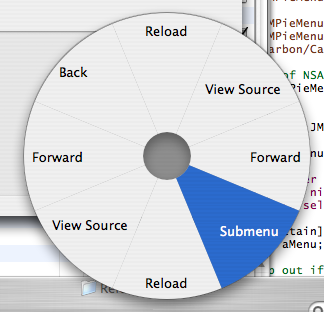
\includegraphics[scale=0.5]{30-10-15-01}
  \caption{Esempio di Pie Menu}
\end{figure}

\section{Lezione del 05-11-15}

\subsection{Pubblicit\`a}

Oggi la pubblicit\`a \`e normale, tempo fa no. Fa parte del \textit{modello di business standard}. Questo viene applicato in un servizio gratis principalemente, in quanto la pubblicit\`a permette di sostentare il sito.

\paragraph*{Reazione degli utenti}Agli utenti non piace la pubblicit\`a, in quanto si frappone ai loro obiettivi di navigazione. Una misura sul click della pubblicit\`a web \`e dello $0,4\%$. \`E importante avere un buon posizionamento all'interno del sito web come nei motori di ricerca, in modo tale che il messaggio pubblicitario sia il quanto pi\`u efficace possibile.

\subsubsection{Posizionamento}Un buon posizionamento, in prima analisi e considerando le coordinate assolute sulla pagina \textit{la colonna di sinistra} \`e un buon punto di posizionamento, seguito dalla striscia\textit{ top della pagina}, dalla \textit{colonna di destra} e infine con la pubblicit\`a \textit{in fondo la pagina} (viene visualizzato 10 volte in meno).
La pubblicit\`a messa \underline{vicino} a contenuto interessante viene visualizzata maggiormente.
La taglia della pubblicit\`a influisce relativamente sulla visibilit\`a del messaggio.

\subsubsection{Metodi di promozione del messaggio pubblicitario}\`E da evitare assolutamente (ordinato in modo crescente) che il messaggio pubblicitario\footnote{Percentuale di non-gradimento}:
\begin{enumerate}

\item Suoni automaticamente ($79\%$)
\item Sia in movimento ($79\%$)
\item Lampeggi ($87\%$)
\item Occupi la maggior parte della pagina ($90\%$)
\item Si sposti sullo schermo ($79\%$)
\item Non dica di cosa si tratti ($92\%$) $\to$ gambling click
\item Copra quello che si sta cercando di leggere ($93\%$)
\item Non abbia un modo chiaro per toglierlo ($93\%$)
\item Cerchi di farsi cliccare sopra ($94\%$)
\item Si carichi lentamente ($94\%$)
\item Sia un pop-up ($95\%$)

\end{enumerate}
Quindi devono essere usati altri ``effetti speciali''.
Le immagini pubblicitarie rispondono alle dinamiche delle immagini nel web, rimanendo in serie B. Questo a causa dell'effetto \textit{``zapping''}, in cui viene applicata da parte del cervello umano una meccanica automatica in cui vengono ``eliminate le scocciature''. Questo effetto viene accentuato se l'immagine \`e una pubblicit\`a.
La regola dello zapping si applica anche al testo quando esso \`e troppo grande o troppo visibile, e per superare la barriera dello zapping bisogna andare controcorrente, tramite tecniche studiate a tavolino. In questa maniera vengono saltati gli algoritmi pre-impostati nel cervello attirando l'attenzione degli utenti, riportando gli avvisi pubblicitari in ``serie A''. Quindi \`e necessario \textit{confondere le idee} agli utenti\footnote{Ovvero scardinare gli algoritmi di zapping.}, possibilmente mescolando testo con il contenuto pubblicitario.
I \textit{giochetti web} catturano l'attenzione degli utenti e sono iper-efficaci per la pubblicit\`a, azzerando i timer. \`E importante quindi avere giochi semplici che aiutino anche l'utente con infine l'inserzione pubblicitaria.
Il modo migliore per creare pubblicit\`a \`e il testo, che \`e il miglior \textbf{blending}. Altri effetti se si vogliono usare immagini in maniera efficace \`e creare immagini pubblicitarie in cui le persone (nell'immagine pubblicitaria) guardino l'oggetto d'interesse o di mostrare persone a grandezza naturale, in quanto prima viene analizzato il viso e poi gli organi genitali\footnote{Questo viene in maniera inconscia.}, ed \`e quindi utile mettere la pubblicit\`a in quel punto.

\subsubsection{Contenuto e contestualizzazione}Il contenuto \`e importante, in quanto se mostro oggetti scollegati dal sito l'utente ha un senso di disorientamento/distrazione. Nel sito web questo effetto \`e ancora maggiore, in quanto ogni sito \`e spesso equivalente a una visita specializzata, con una diminuzione del timer dell'utente fino al $-40\%$, e un calo della voglia di ritornare dell'utente del $-80\%$. \`E importante quindi che il contenuto del messaggio pubblicitario sia ``in armonia'' con il sito web anche detto \textit{behaviorial advertising}, cio\`e la ``pubblicit\`a comportamentale'', che cerca di dare un contenuto che interessi all'utente. A differenza di media passivi, nel web \`e possibile diversificare gli utenti, e quindi dare loro pubblicit\`a ``behavioral'' adatta al loro comportamento. L'efficacia di fare la pubblicit\`a behavioral ha un incremento del fattore di interesse di almeno $10x$, fino a $10000x$ volte! La pubblicit\`a behavioral ha anche un effetto benefico sul sito: non solo non subisce gli effetti negativi del \textit{``distracting advertisement''}, ma addirittura in certi casi li ribalta, portando ad un aumento dei timer e della voglia di ritorno.


\section{Lezione del 06-11-15}

\subsection{Ricerca nel sito}

Esiste la ricerca esterna (es Google) e la ricerca interna al sito. La soglia critica per la ricerca interna \`e: per pi\`u di 100 pagine \`e \textit{necessario} usare qualche tool di ricerca, mentre oltre 1000 \`e \textit{cruciale} usare un buon tool di ricerca.

In media, il 100\% usano la ricerca di funzionalit\`a del sito, rendendola molto importante. Gli utenti essendosi abituati ai motori di ricerca li usano per navigare velocemente, ed \`e quindi normale per loro che ci sia in un sito web. Inoltre il problema del \textit{deep linking} evidenzia come un utente possa essere catapultato in una qualsiasi pagina web del sito, e per continuarne la navigazione pu\`o o tornare alla home oppure pu\`o usare la casella di ricarca. Quando accade il deep linking, il 60\% degli utenti usa le funzionalit\`a di ricerca (se c'\`e), mentre il 40\% usa la navigazione normale.

\subsubsection{Ricerca locale}

Google o altri motori di ricerca possono fornire una ricerca in locale (con \textit{site}), i vantaggi sono costo zero nello sviluppo, ma i svantaggi sono che gli algoritmi usati da Google sono progettati per ricerche su larga scala, e non funzionano bene su bassa scala ed inoltre se un utente \`e gi\`a arrivato al sito tramite motore e non ha trovato subito quello che voleva \`e indice che il motore non riesce a dare una buona risposta per quella domanda sul sito. Inoltre i motori di ricerca non indicizzano tutto il sito web, quindi potrebbe essere che il sito non sia completamente indicizzato con un conseguente peggioramento dei risultati di ricerca.

\paragraph*{Creazione di una ricerca interna sul sito}\`E necessario chiedersi che modalit\`a di ricerca preferiscono gli utenti, e la funzionalit\`a di ricerca normale dev'essere molto simile a quella dei motori di ricerca, con un \underline{box testuale} per la ricerca e un \underline{pulsante} con la scritta ``Search''\footnote{In italiano ``Cerca''.} o con l'icona della lente per effettuare la ricerca.
Il principio \textbf{``less is more''}, afferma che \`e meglio aver qualcosa di pi\`u semplice, e questo principio \`e applicabile anche alla semplicit\`a con cui si devono presentare gli strumenti di ricerca.


\paragraph*{Ricerca vincolata}La ricerca classica nei siti pu\`o essere presentata con la cosiddetta \textit{constrained search}, dove tipicamente dev'essere data in aggiunta alla ricerca classica. I pro della ricerca vincolata data in aggiunta alla ricerca classica \`e che \`e molto gradita dagli utenti, ma per contro occorre stare attenti a come si implementa, dato che non fa parte dei motori di ricerca classici. Esistono due modi di fare ricerca vincolata: in modo statico e dinamico:
\begin{itemize}

\item Ricerca Dinamica: appena l'utente riempie il campo parte la ricerca
\item Ricerca Statica: l'utente deve premere il pulsante per effettuare la ricerca

\end{itemize}
Il problema della ricerca statica \`e che il pulsante non essendo standard pu\`o mettere in confusione l'utente. Per contro la ricerca dinamica richiede qualche secondo (in quanto esegue ogni volta la ricerca) causando che molti utenti si stufino aspettando il risultato. La ricerca vincolata sembra essere la ricerca migliore, ma dipende da quanti vincoli ci sono nella ricerca: se i vincoli sono 1, la dinamica \`e superiore, ma se aumentano c'\`e una dilatazione del tempo, con un aumento della attesa per ogni vincolo settato e un carico maggiore nel server. \`E anche possibile adottare una soluzione ibrida: viene lanciata automaticamente la ricerca quando tutti i vincoli sono stati riempiti.
Una funzionalit\`a molto rischiesta dagli utenti \`e la possibilit\`a di fare sorting dei risultati in maniera \underline{bidirezionale}.


\`E necessario saper gestire quando non ci sono risultati nella ricerca, e possiamo dire che non ci sono stati risultati o che ci sono stati zero risultati. Dire all'utente che non ci sono stati risultati lo confonde e lo porta a pensare che la funzione di ricerca non vada. Dare 0 risultati \`e meglio in quanto l'utente ne viene a conoscienza e capisce che non ci sono risultati. Rohe oltre a dire ``Less is more'' diceva anche ``God is in the details'', quindi \`e importante curare anche i dettagli. Ottenere 0 risultati in una ricerca \`e come ottenere un codice 404, detto anche ``dangling link''.

\section{Lezione del 12-11-15}


\paragraph*{Modalit\`a di presentazione dei risultati}Nel presentare i risultati di ricerca ad un utente solitamente \`e meglio adottare una presentazione lineare. Una modalit\`a alternativa \`e a griglia, che presenta il vantaggio di contenere pi\`u informazione e di fornire una rappresentazione compatta a livello visivo, ma tende a far perdere la rilevanza dei risultati, causando disorientamento all'utente con conseguente perdita di tempo.

\subsubsection{Struttura del box search}\`E importante tenere conto della grandezza della casella di ricerca e del modo di cercare degli utenti: si \`e infatti notato che rispetto alle prime ricerche (che si basavano su keyword) ora si \`e passati a query pi\`u complesse. La lunghezza media consigliata per la grandezza di una casella di ricerca \`e di almeno 30 caratteri, in quanto il 90\% delle query presenta una lunghezza simile. In caso il box di ricerca sia troppo piccolo si hanno diversi problemi:
\begin{itemize}

\item Effetto psicologico: lo stress dell'utente aumenta proporzionalmente in base alla quantit\`a di testo non visualizzato nel box di ricerca (1\% di stress in pi\`u per ogni carattere)

\item Effetto perverso sulla ricerca: su un box piccolo gli utenti tendono a scrivere meno quindi il motore ha una ricerca meno precisa e i risultati ottenuti sono pi\`u scarsi.

\end{itemize}



\section{Lezione del 13-11-15}

\subsubsection{Assistenza multimediale}

La assistenza multimediale viene anche detta ``Ricerca 2.0''. Crea un danno al sito del -42\%. L'utente di fronte a un Human Digital Assistant diventa pi\`u esigente e si aspetta un'interazione maggiore e per migliorarne l'esperienza \`e meglio scegliere un avatar che non ricordi una forma umana.
Con l'assistenza multimediale il rumore di fondo \`e la chiave per creare negli utenti una sensazione positiva, rendendo pi\`u caldo e pi\`u gradevole un sistema a lato utente.

\subsection{Visibilit\`a del Sito}

\`E essenziale essere nella top ten dei motori di ricerca per poter essere ``trovati'' dall'utente.

\subsubsection{SERP}

Il posizionamento di un sito web all'interno di un risultato di ricerca \`e molto importante. I primi 10 risultati di ricerca assorbono il 95\% dei click.
Percentuale dei click in base alla posizione:
\begin{itemize}

\item Prima posizione: 51\%
\item Seconda posizione: 16\%
\item Terza posizione: 6\%
\item Quarta posizione: 6\%
\item Quinta posizione: 5\%
\item Sesta posizione: 4\%
\item Settima posizione: 2\%
\item Fino al decimo posto: 2\%. Questo a causa dell'effetto Jearsy (o effetto Malabrocca)

\end{itemize}


\section{Lezione del 26-11-15}

\paragraph*{Ricerca google}Nella pagina di ricerca google la sezione immagini nella ricerca normale \`e stata introdotta perch\`e si \`e visto che le immagini hanno effetto sospensivo e i timer si rilassano.

\subsubsection{Tecniche per il calcolo del punteggio di una pagina}
Esistono diverse tecniche per entrare in classifica nei motori di ricerca, ed esse possono essere: spamdex\footnote{spam index}, SEO, SEP.

\paragraph*{Calcolo del punteggio di una pagina}Il calcolo del punteggio di una pagina viene diviso in base al tipo di contenuto, ovvero se testo o se immagini. Se il contenuto \`e testo allora si parla di \textit{TFIDF}\footnote{Detto anche TF-IDF, acronimo di Term Frequency Inverse Document Frequency.}, e serve a capire quando una parola \`e importante per una pagina. La frequenza inversa del documento si calcola con la frequenza della parola nell'insieme dei documenti, scalato logaritmicamente.
Ad esempio:
\begin{itemize}

\item Avendo un sito di 1000 pagine, ipotizzando ``il'' appaia in 980 pagine $\to$ 98\% di frequenza $\to$ IDF di $\log(\frac{1}{0,98}) = 0,008$
\item Avendo un sito di 1000 pagine, ipotizzando ``pippo'' appaia in 100 pagine $\to$ 10\% di frequenza $\to$ $\log( \frac{1}{0,1}) = 1 $
\end{itemize}

Riassumendo, quando al motore di ricerca gli viene fatta una query di un certa parola $p$, egli prende tutte le pagine dove appare $p$ e calcola il loro TFIDF e se sono presenti pi\`u match allora ne calcola la loro somma.

\paragraph*{Keyword}\`E quindi importante definire delle \textit{keyword}, per cercare di alzare il loro TFIDF. Esistono diverse tecniche per inserirle all'interno di un sito web, e sono:
\begin{itemize}

\item \textbf{Body spam}: si inseriscono le parole nel body della pagina HTML (semplice ed efficace, ma ha lo svantaggio che \`e un effetto visibile all'utente)
\item \textbf{Title spam}: il contenuto viene toccato meno o comunque su una parte di pagina a cui l'utente non fa molto caso
\item \textbf{Meta tag spam}: le keyword vengono scritte dentro il contenitore apposito. Questo ha il vantaggio di non toccare il contenuto della pagina web, ma essendo abusato il punteggio dei motori di ricerca per questo meta-tag \`e molto basso
\item \textbf{Anchor text spam}: \`e una tecnica in cui le keywords vengono inserite nell'anchor text. Questo porta come vantaggio la generazione di punteggi speciali, ed ha come particolarit\`a che le Keywords su un link vengono aggiunte anche nel target del link. Il bonus inoltre viene dato con meno limiti per TFIDF.
\item \textbf{URL Spam}: le keyword vengono aggiunte direttamente nell'indirizzo web, in quanto alcuni motori analizzano anche gli indirizzi delle pagine e danno bonus simili a quelli dell'anchor text spam.

\end{itemize}

\`E importante tenere conto anche della forma con cui le keywords vengonono inserite in una pagina web. Esistono diverse tipologie:
\begin{itemize}

\item Repetition: si ripete la parola pi\`u volte
\item Dumping: si interiscono tantissimi termini usati poco, anche se non c'entrano nulla
\item Weaving: si prendono pezzi di pagine web e si inseriscono al loro interno le kaywords volute (in maniera randomica)
\item Stitching: si esegue il paste\&copy di frammenti di pagine web diverse e le si ri-assembla
\item Broadening: si inseriscono i sinonimi alle keywords, in modo da coprire meglio il campo delle query su cui si viene intercettati

\end{itemize}

Da tenere conto \`e anche la scelta delle keyword: si deve basare su cosa ``vogliono'' gli utenti.

\section{Lezione del 27-11-15}

%stiamo finendo di vedere le tecniche di hiding

\paragraph*{Cloacking}Il cloacking \`e la strada pi\`u rapida per il ``ban'' dai risultati di ricerca di google.

Con il cloacking si distingue tra gli utenti normali e gli spider di ricerca, mostrando pagine diverse. Questa tecnica \`e molto efficace e difficile da scoprire, perch\`e la pagina dev'essere confrontata da un umano.

\subsubsection{Componente ipertestuale}
Una buona parte di punteggio viene data dalla forma del web e dalla sua \textit{topologia di rete}.
Uno strumento usato \`e il pagerank, che utilizza la seguente formula:

\[ \pi_v = \sum_{(w,v) \in E}\frac{\pi_w}{d_v} \]

Dova la sommatoria totale \`e pari a 1.

La formulazione avviene attraverso le catene di Markov e utilizza random walks. \`E quindi il processo Markoviano corrispondente a un link. Questo modello siccome corrisponde a un attore che naviga scegliendo i link a caso nel web\footnote{Questo viene anche detto anche in gergo web ``scimmia'' (random surfer).}, e non corrisponde alla navigazione reale di un utente nel web, crea discrepanze tra quello che si fa realmente e quello che viene calcolato con il PageRank.

Le \textit{spider traps} sono delle trappole per gli spider dei motori di ricerca dove un si viene ``intrappolati'' in un sito e non riesce pi\`u ad uscirne. Questi avvenimenti sono molti frequenti, per esempio:
\begin{itemize}

\item Lo spider tenta di ``catturare'' un calendario online (quindi continua a percorrere tutto il calendario)
\item Problema island: in cui non \`e possibile decidere quale pagina \`e la pi\`u importante

\end{itemize}

Si \`e deciso quindi di cambiare la formula del PageRank, cambiandola con la cosidetta \textit{componente del teletrasporto}, che considera non solo la parte del punteggio tramite i link, ma anche quella del ``teletrasporto'', che assegna il punteggio in maniera democratica seguendo una determinata probabilit\`a.

\[ \pi_v = (1- \epsilon) ( \sum_{(w,v) \in E}\frac{\pi_w}{d_v}) + \frac{\epsilon}{N} \]

Questo permette di ``teletrasportare'' lo spider in un'altro punto casuale del web, impedendo di entrare in loop e di sballare i risultati del PageRank. \`E importante notare che il parametro $ \epsilon $ permette di gestire il livello di ``democrazia'' dei punteggi\footnote{$\epsilon$ pu\`o avere valore al pi\`u 1.}. 

%\paragraph*{Totalrank}\`E stato sviluppato un altro algoritmo, che \`e la media di tutti i valori possibili del ``teletrasporto''. Il suo costo \`e lo stesso del pagerank.\newline

%\[ T = \int_{0}^{1}  -- formula mancante
%--------------------

Un altro problema sono le ``dead ends'', dove si crea una struttura in cui gli altri siti puntano ad un sito che non fa ``uscire'' altri link, facendo aumentare il rank del sito che non punta ad altri. Per ovviare a questa situazione, Google e Bing hanno cambiato la struttura web e il modo di vedere i link all'interno dei loro sistemi. Questo complica ai SEO i calcoli che devono essere fatti per poter promuovere il proprio sito web.


Sono quindi presenti due fattori importanti: i link entranti in un sito e i link uscenti. I link entranti nel sito aumentano molto il punteggio, ed esistono delle tecniche di base:
\begin{itemize}

\item \textbf{Infiltration}: consiste nell'``infiltrarsi'' in vari siti e cercare di inserire un link al proprio sito.
\item \textbf{Honey Pot}\footnote{In italiano ``Barattolo del miele''}: consiste nel creare contenuto ``appetibile'', e quindi ricevere poi natualmente degli incoming link. Questo metodo dovrebbe essere il moto giusto per aumentare il proprio PageRank (tecnica etica). Nella pratica viene usata in modo poco etica, eseguendo il paste\&copy intelligente dal contenuto di altri siti.
\item \textbf{Link Exchange}: consiste nel mettersi d'accordo con altri per scambiarsi i link
\item \textbf{Resurrection}: consiste nel riprendere un dominio ``in vendita'' o non pi\`u usato. Questo perch\`e il dominio comunque detiene un certo punteggio.

\end{itemize}

Mentre per i link esterni si hanno dinamiche diverse. Il comportamento di PageRank infatti non ha avuto dinamiche prevedibili per i link esterni, questo a causa della tecnica del teletrasporto degli spider. Ci\`o si ripercuote nelle tecniche pi\`u avanzate:
\begin{itemize}

\item \textbf{Spam Farm}: creazione di una struttura apposita per l'incremento del punteggio tramite link. Una spam farm ottimale \`e: una pagina target e le altre che puntano in maniera bidirezionale a essa. Questa sfrutta una propriet\`a detta \textit{reachbility}, che \`e essenziale per gli spider. Un altro aspetto importante per questo \`e creare le cosiddette \textit{alleanze} tra siti, che permettono di mediare il PageRank tra i due siti se esse sono \textit{profonde}, mentre si ottiene pi\`u del massimo se esse sono di tipo \textit{superficiale}.

\section{Lezione del 03-12-15}

\`E possibile espandere le alleanze non solamente a due siti, ma anche a un numero maggiore. Esiste non solo la generalizzazione \textit{ring}, ma \`e possibile creare un anello bidirezionale, detto anche \textit{cuore completo}, che presenta varie propriet\`a.

\subsubsection{Comportamento dei motori di ricerca}I motori per controbattere le alleanze tentano di identificare e comprendere le strutture ad anello. Ma se se si formano l'unione delle pagine, creando un grafo fortemente connesso (ovvero da ogni pagina arrivo a un'altra) si \`e in grado di aggirare questo problema. I grafi fortemente connessi sono anche utili per la \textit{reachability}, una ottima propriet\`a per un'alleanza web.

I motori di ricerca ora cercano unioni di siti tra grafi fortemente connessi, ma maggiore \`e l'unione dei siti pi\`u \`e difficile per i motori di ricerca trovare queste alleanze.

\paragraph*{Sequenza A003030}Il modo migliore per creare un'alleanza si definisce tramite la sequenza \textit{A003030}\footnote{Trovabile online nella ``grande enciclopedia delle sequenze''.}. Questa sequenza \`e molto potente, e gi\`a in 10 siti alleati il motore di ricerca non riesce a identificare eventuali alleanze. I motori di ricerca per evitare ci\`o adottano delle contromisure pi\`u sofisticate. Attualmente in Google vengono applicate due contromisure principali:
\begin{itemize}

\item Viene rimossa la parte del ``Teletrasporto'' del PageRank e viene confrontata con la versione con Teletrasporto, ottenendo il \textit{valore di massa di spam relativa}, valore che permette di identificare eventuali alleanze. Infatti se il valore di Teletrasporto \`e molto grande allora i motori di ricerca sono in grado di percepire che un sito sta tentando di spostare il ``flusso'' verso di se. Il rate di successso di questa tecnica \`e del valore del $95\%-100\%$.

\item Utilizzando la struttura del web\footnote{\`E una struttura ad altissimo livello.}, che assomiglia a un papillon, \`e possibile effettuare una contromisura efficace a basso costo computazionale. Se analizzando la struttura del sito web si trova che essa differisce troppo dalla struttura media degli altri siti web allora \`e probabile che ci sia qualcosa che non va. La media viene effettuata su una ``lastra'' dei link entranti da Google, da cui \`e possibile tracciare una norma e da li notare i siti che si discostano da essa. Questa tecnica produce molto successo.

\end{itemize}

\subsubsection{Misure attuali del PageRank}
La misura del PageRank, come gi\`a visto, \`e dato in parte dal flusso e in parte dal trasporto. Si \`e cercato soprattutto di migliorare la qualit\`a della ricerca complessiva soprattutto sul fattore di ``teletrasporto'' ($\frac{\epsilon}{N}$).
Cambiando il teletrasporto \`e possibile ottenere valori pi\`u sensati, ottenendo una formula che genera un rank molto migliore. Questo teletrasporto generalizzato viene detto \textit{personalize PageRank}, in cui cio\`e i nodi non sono tutti uguali, ma sono pesati. Questo causa al modello di diventare pi\`u simile a una navigazione reale.

Quindi in base all'utente sono presenti diverse preferenze. Se l'utente \`e Google allora potrebbero venire penalizzati alcuni siti in base a delle scelte arbitrarie, incorporandole poi nell'algoritmo di teletrasporto. Il PageRank usato da Google attua questa politica, e alcune correzioni vengono fatte a mano, e non \`e una misura assoluta (e tantomeno quindi ``democratica'' nel senso di oggettiva e imparziale). Ad esempio SearchKing \`e stato per motivi commerciali penalizzato da Google Stesso.

\paragraph*{PageRank personalizzato}Per l'utente singolo \`e possibile calcolare un PageRank ``personalizzato''. Questo comporta un costo molto oneroso, in quanto deve essere creato un PageRank per ogni utente navigante nel web. Se per esempio nel web ci fossero $N$ pagine e fossero possibili solamente il valore ``mi piace'' e ``indifferente'' avremmo $2^N $ personalizzazioni possibli. In realt\`a il pagerank personalizzato \`e linearmente componibile, ergo \`e possibile combinare pagerank personalizzati senza ricalcolo, quindi da $2^N $ si passa a $N$ pagerank personalizzati che comunque rimane la taglia del Web. Per ovviare a questo problema Google esegue il \textit{topic pagerank}, creando profili che ``approssimino'' varie tipologie di utente, in base agli argomenti visitati dagli utenti, e su di esse viene \textit{precalcolato} il PageRank personalizzato. In questo modo dai profili ``grezzi'' \`e possibile creare dei profili astratti in base agli interessi, da cui \`e possibile quindi creare una pubblicit\`a migliore.

Il PageRank personalizzato \`e compatibile con tutte le contromisure (massa di spam relative, e tutte le tecniche basate sulla struttura web).


\subsubsection{Funzionamento dei motori di ricerca}

Fino a poco tempo fa, per studiare i sistemi di ranking ci si basava solamente sulla ``bont\`a'' di un sito. Al giorno d'oggi, le misure sono cambiate. Le contromisure erano viste come una ``patch'', un aggiustamento, piuttosto che una caratteristica di prima classe.

La visione pi\`u recente dei siti web si basa sul fatto che nel ranking esistono due lati: quello buono e quello cattivo, e ogni pagina ne presenta un tratto.
\`E necessario oltre al lato buono di una pagina darne anche un lato ``cattivo'', ed \`e necessario sviluppare una maniera automatizzata per determinare ci\`o.

Prendendo ispirazione dalla divinit\`a romana Giano (bifronte) e calandolo nel lato tecnologico predono vita i \textit{grafi di Giano}\footnote{Detto Janus graph.}, dove ogni nodo (pagina web) non ha un valore, ma presenta due valori: una parte ``positiva'' e una ``negativa''. Questi grafi bipesati sono le ``due facce'' di un nodo, che vengono combinate nel calcolo del rank finale per generare ricerche adeguate.
Considerando $R_{GOOD}(G^+)$ il lato buono e $R_{BAD}(G^-)$ si pu\`o considerare il tutto come una combinazione lineare:

\[ \alpha \cdot R_{GOOD}(G^+) - \beta \cdot R_{BAD}(G^-) \]

Il problema di tutto ci\`o si riversa nel fatto che ora dovrebbero esistere due funzioni di ranking, un ``anti-pagerank'', avendo il doppio dei problemi e il doppio dei pesi: $W^+$ e $W^-$.

\paragraph*{Gestione del doppio ranking}Per evitare di avere due algoritmi di ranking \`e possibile avere una estensione del ranking attuale, che si identifica come la \textit{estensione di Giano}. Essendo l'una lo specchio dell'altra risultano essere anche lo specchio della struttura web, e quindi \`e possibile ragionale sul web ``al rovescio'', generando un web duale $G^\#$. Dalla misura ``buona'', si ottiene la sua estensione:

\[ R^J = R(G^+)-R((G^\#)^-) \]

Dove quindi con la stessa formula si ottiene la misura di $G^\#$.

\section{Lezione del 04-12-15}

Per avere informazioni utili su $W^-$ si \`e cercato in diversi posti.

\paragraph*{Email}L'``email space'' \`e uno spazio informativo virtuale molto ricco, in vario modo sottostimato finora dato che tecnicamente \`e distaccato dalla struttura Web (spazio URL-based). Notando lo spazio delle mail \`e possibile notare come siano presenti delle somiglianze con la struttura del web: un nodo \`e costituito da un indirizzo email, e si crea un link diretto dall'indirizzo email $E1$ all'indirizzo email $E2$. Sono naturalmente possibili modellazioni pi\`u sofisticate: ad esempio, i nodi potrebbero essere le singole email, o email threads etc etc.

\paragraph*{Spazi email e web}

Ogni volta che un'email menziona un URL, viene creato un link corrispondente da quell'indirizzo email alla pagina web rappresentata da quell'URL, oppure, quando da una pagina web menziona un certo indirizzo email, viene fatto un link da quella pagina a quell'indirizzo, creando un ``super-web'' molto pi\`u grande di quello precedente.

Spesso si parla della ``popolarit\`a'' di una pagina web: ora, l'integrazione degli spazi email porta questo concetto ancora pi\`u in l\`a.

\paragraph*{Gestione del Janus Graph per l'email}

Le mail vengono applicate nella considerazione delle due ``facce'':

\begin{itemize}

  \item[Buona] si possono considerare misure positive di ``activeness'', a seconda di come/quando le email inviate ad un certo indirizzo ricevono risposta o meno. Come nel classico spazio web, quest'informazione si pu\`o integrare con altre caratteristiche come l'et\`a (quando l'account \`e stato creato) e la history (es. calcolare la \textit{misura integrale} dell'activeness nel tempo).

  \item[Cattiva] negli indirizzi mail la ``cattiveria'' \`e associabile allo spam. Ogni qual volta una email viene classificata come spam, a quell'indirizzo e a tutti gli URLs/URIs dentro quella mail pu\`o essere assegnata un po' di ``cattiveria''. Ogni volta che una mail viene segnalata come spam viene segnata con un valore ``maggiore'' di cattiveria. Uno dei motivi per cui Gmail \`e stata acquistata da Google \`e per ottenere un maggior numero di informazioni possibili. Ogni segnalazione di spam su Gmail si riverbera sui risultati di ricerca.

\end{itemize}

I motori di ricerca odierni vanno oltre la ``scatola chiusa'' del web, collegandosi ad altri mondi. Gli ``attacchi'' nel mondo delle mail son pi\`u difficili da fare, in quanto le mail sono pi\`u di ``natura sociale''. Inoltre sono stati innalzati dei ``muri'' per la creazione degli indirizzi mail (vedasi  i CAPCHA). I CAPCHA presentano un problema di usabilit\`a per gli utenti, ma viene messo per garantire di avere un certo controllo sull'ambiente, avendo la garanzia di avere servizio usato da umani.
Il vantaggio del mondo email \`e che pu\`o essere pi\`u facilmente \textit{tracciato}, al contrario delle pagine web. \`E molto pi\`u facile distinguere tra comportamenti \textit{reali} e \textit{artificiali}.

\paragraph*{Altri spazi in cui trovare l'informazione}

Un altro passaggio ulteriore \`e stato di non considerare solamente i sistemi informativi, ma anche i sistemi sociali: SIS\footnote{Social Information System.}. Un problema che si incontra quando si tenta di estendere tutto ci\`o considerando anche le persone sono le identit\`a. Un information system dove a ogni oggetto viene assegnato uno UID\footnote{User Identifier.}, rispetta il cosidetto \textit{identity mapping}. Infatti con UID diversi con altra probabilit\`a si sta parlando di utenti diversi, e quindi tenendo sempre il modello astratto semplice e modulare, il ranking pu\`o essere fatto agire direttamente su di un SIS. Esistono diversi modi per migliorare il ranking:

\begin{itemize}

\item Social rankings: in modo canonico quasi ogni ranking usa flussi basati su cammini. A ogni path flow si pu\`o facilmente assegnare una ``taglia sociale'', corrispondente alla taglia dell'ambiente sociale (quanti utenti) che lo ha creato. \`E quindi facile produrre un social Pagerank come anche altri social rankings!

\item Social Pagerank: l'attuale ranking di Google gi\`a incorpora alcune componenti di Social Pagerank. Quindi l'acquisto di pi\`u domini dalla stessa persona e il tentativo di utilizzare le tecniche di Spam Farm e simili valgono molto poco. Attualmente sono in sviluppo anche tecniche di Social Pagerank che si basano sulla analisi della scrittura dei testi (come per esempio i blog). Ogni UID viene assegnato alle pagine in base all'autore: link agli articoli di uno stesso autore sono poco significativi, mentre link allo stesso dominio ma di autori diversi hanno un maggior valore.

\end{itemize}

Dopo l'utilizzo delle mail, si sta migrando verso la cosiddetta sociosfera informativa, dove ogni tipologia di sito ha un ranking basato su determinate azioni. Per esempio in un Wiki il rank varia in base alle diverse modifiche eseguite da pi\`u autori su una voce, o in Google Play Store un'app ha posizione in base alla sua discussione e altri fattori.

\subsection{Nomi nel Web}

Esistono due tipologie di nomi: lato sociale e lato tecnico.

\subsubsection{Lato sociale}

\`E fondamentale scegliere un buon nome per un indirizzo web. Ci sono alcune regole che massimizzano il potenziale successo di un sito. In media il 10-20\%, ma \`e possibile arrivare fino ad un +40-50\% di influenza.

Esistono diverse regole per la scelta di un giusto nome:

\begin{enumerate}

\item Usare nomi corti
\item Nome unico e non simili con altri nomi, non scegliere un plurale quando il singolare \`e gi\`a preso
\item Prendere il dominio .com. Questo ha un impatto medio del +4.5\%
\item Dovrebbe essere facile da memorizzare e scrivere
\item Meglio scegliere parole esistenti pittosto che inventarsene di nuove. In ogni caso, se si usano parole nuove o acronimi, conta il rapporto tra parole ``standard'' e quelle nuove: pi\`u alto \`e il rapporto, meglio \`e. Il range va dal +1.5\% a -5\%.
\item Bisogna riporre attenzione al suono. La regola intuitiva \`e che deve ``suonare bene'', dev'essere piacevole e armonioso. Nella pratica questo \`e stato calcolato: in inglese i nomi che cominciano con una vocale funzionano bene (circa +3.7\%). Le semivocali (r, j, y, w) funzionano bene (+2.9\%). Le consonanti di tipo f, v, s, z funzionano ancora meglio (+3.3\%). Le consonanti come p, k, t funzionano meglio delle restanti (+1.9\%). Suoni associati con parole brutte (tipo ``uh'') creano danno al sito fino ad un -44\%. In altri contesti, ad esempio materiale adulto, generano vantaggi al sito fino ad un +7\%.
\item Niente trattini. Si ha un impatto pre-sito del -3\%
\item La regole del ``nessun numero'' (regola che si trova in giro su internet) \`e falsa. Anzi, i numeri aiutano, con un impatto del +8.2\%.
\item \textbf{Importante}: attenzione a come controllare se un nome \`e libero o no. Ci si crea una lista di nomi liberi, e si scarta quelli occupati per far rimanere solo quelli liberi. \`E importante fare attenzione perch\`e questo ciclo pu\`o diventare sbagliato, in quanto nei siti di vendita dei siti di domini potrebbero raccogliere i nomi che si cercano. \`E importante fare attenzione e usare \textbf{internic}, che \`e un servizio governativo e istituzionale, che ha delle politiche di privacy.

\end{enumerate}

\section{Lezione del 10-12-15}

\subsubsection{Lato tecnico}

\paragraph*{URI}Gli URI si distinguono dagli URL, e non vanno confusi. Gli URI sono un sovrainsieme degli indirizzi web. Ad esempio un www.sito.it non \`e un URI corretto, e non esiste negli standard: la voce corretta sarebbe http://www.sito.it. URI sono anche indirizzi mail.

\paragraph*{Differenze tra URIs, URLs, URNs}Gli URL stanno per \textit{Uniform Resource Locator}, ovvero gli URL attraverso la loro rappresentazione ci indicano il modo per arrivare alla risorsa. Quindi gli indirizzi ``http://...'' sono URLs.

URNs significante \textit{Uniform Resource Name} sono identificatori che restano unici e persistenti che durano anche quando la risorsa cessa di esistere o non \`e pi\`u disponibile.

Un URI pu\`o essere \textit{assoluto} o \textit{relativo}. Se assoluto \`e gi\`a ``completo'' cos\`i com\`e, mentre se relativo non \`e completo, per essere completato deve essere trasformato in un URI assoluto tramite informazione derivante dal contesto.

\paragraph*{Struttura di un'URI}La loro struttura di un'URI si rappresenta nella seguente maniera:
\begin{verbatim}
Struttura:parte-dipendente-dallo-schema
\end{verbatim}

Lo schema \`e quello che definisce la \textit{semantica} (il significato) dell'URI. Gli URI in generale possono essere parte di due grosse famiglie: possono essere gerarchici quando la loro forma \`e:
\begin{verbatim}
Schema :// authority path ? query
\end{verbatim}

Le autortiry, rappresentano l'\textit{autorit\`a}, ovvero \`e l'elemento che indica l'autorit\`a, e che risponde in caso di problemi. La \textit{path}, ``cammino'', si compone di zero o pi\`u segmenti, ognuno della forma:
\begin{verbatim}
/segmento
\end{verbatim}
Nota: lo hash(\#) \`e un carattere riservato per gli URI, e serve per delimitare l'URI di un oggetto con un identificatore di un frammento interno alla risorsa considerata.
La \textit{query} presenta l'informazione interpretata dalla risorsa.

Gli URI possono essere anche opachi, quando manca il simbolo ``/''. Per esempio:
\begin{verbatim}
mailto:director@cnn.com
\end{verbatim}
rappresenta un URI opaco. Nota che anche in questo caso \`e possibile passare argomenti nella query. Altri esempi di URI possono essere i numeri di telefono (tel) o fax (fax) e altri.

\paragraph*{URNs}Gli URN sono indirizzi web di tipo opaco, e significa \textit{Uniform Resource Names}, e hanno la forma tipica:
\begin{verbatim}
urn:NID:...
\end{verbatim}
Per esempio, gli identificativi ISBN sono URN, rappresentano un nome di un libro, che non \`e detto che sia ancora disponibile. \newline


Gli URI, URL, URN usano gli ASCII, ma dato l'espansione del suo utilizzo di \`e passato dall'URI all'IRI\footnote{Che sta per Internationalized Resource Indentifiers}, che adotta un set di catatteri pi\`u ampio. Da qui sono nati gli IDN, che possono essere usati anche nelle estensioni web.

Ci\`o ha portato ad un maggior rischio agli \textit{attacchi omografici}. Infatti \`e possibile che siano presenti indirizzi graficamente uguali ma i simboli provengono da altri alfabeti.

\paragraph*{Problema di Opacit\`a degli URI}Il significato di:
\begin{verbatim}
http://www.sito.it/a/b.html
\end{verbatim}
non indica necessariamente che il sito sia in italiano, o che il sito si trovi in italia, in quanto questi indicano solamente dei nomi. Queste informazioni infatti non sono fornite dall'URL. L'URL rappresenta una \textit{stringa opaca} da cui non \`e lecito inferire alccuna propriet\`a della risorsa corrispondente. HTTP fornisce metodi (\textit{content negotiation}) per capire il formato dati. La parte finale dell'URL non \`e attendibile.

Un altro problema riguada i TLD (\textit{Top Level Domain}). La tendenza \`e di sovradimensionare i TLD, creandone troppi. La proposta \`e iniziata con creare nuovi TLD per categorizzare siti per adulti o porno, e tutto ci\`o spinto da aziende che vendono domini. Questo causa il forzare tutto il contenuto all'interno di un certo TLD (nel caso pensate), o di consigliarlo (nel caso leggero). Anche se i costi tecnologici sono bassi, il \textit{costo sociale} nel caso leggero non presenta alcun vantaggio e nel caso pesante l'interpretazione del WHO diventa pi\`u informativa, eliminando i vari problemi di categorizzazione (ma in realt\`a no) perch\`e usare l'URL per scopi che non sono i suoi, forzandoci informazione che non dovrebbe stare l\`i, \`e pura stupidit\`a tecnica.


\subsection{Torre di babele}

Al MIT vengono creati dei sistemi intelligenti come ``Manda una rosa alla mia ragazza'', dove si veniva trovato un sito web di vendita fiori e venivano inviate delle rose all'indirizzo salvato. Questi sistemi non funzionano bene in quanto ci sono problemi con la raccolta di informazioni nel web.
Un sistema simile viene eseguito con la RIIA (tipo SIAE italiana) per la ricerca di musica piratata. Questi bot per\`o potrebbero ricadere nello stesso caso del MIT.

\section{Lezione del 11-12-15}

Le informazioni vengono scritte tramite HTML, che \`e semplice ma molto limitato. Si \`e quindi passati a un nuovo metodo, tramite XML, che rende l'strazione dei dati dal web pi\`u semplice. XML \`e semplice e flessibile\footnote{Esistono molti dialetti.} ed \`e stato creato proprio per rispondere a questa esigenza. Purtroppo la stessa flessibilit\`a di XML \`e anche allo stesso tempo la sua pecca, in quanto manca una funzionalit\`a fondamentale dell'aggregazione dell'informazione: infatti il potere del web sta nel suo carattere distribuito e l'enorme potenziale sta quindi \textit{nell'aggregazione} di tutte queste risorse. L'aggregazione XML funziona bene quando si usa \textit{lo stesso} dialetto XML, ma quando cominciano a esistere diversi dialetti multipli non si hanno pi\`u gli strumenti tecnici per l'aggregazione: XML fallisce nel modello \textit{open-world}.

La struttura dati di base di XML non \`e una struttura dati fatta per l'aggregazione\footnote{La struttutra dati XML \`e fatta ad albero.}, e l'unione di due alberi porta alla creazione di una foresta, detta anche collezione di documenti XML. Per superare questo problema si \`e cercato di rendere possibile l'aggregazione automatica dell'informazione e di rendere possibile il \textit{ragionamento automatico} su tale informazione, creando il web semantico. Il significato di web semantico significa aggiungere del significato al web. \`E necessario quindi avere una sorta di \textit{pesce di Babele} per il Web. Da qui la nascita di \textbf{RDF}\footnote{Significa Resource Description Framework}, che si occupa di descrivere relazioni e concetti, ovvero dei ``metadata''\footnote{Ðefinizione: metadata is the data that I forgot to put in the first place.} (dati sui dati, dati di livello superiore).

\paragraph*{RDF}Tecnicamente \`e un ``enriched entity-relationship'' knowledge model. \`E presente una grammatica di base, dove una ``frase'' \`e composta da:
\begin{itemize}

\item soggetto
\item predicato
\item complemento oggetto
  
\end{itemize}
La ``frase'' \`e il mattone principale di RDF, e in un certo senso, stiamo insegnando al web l'inglese. L'RDF pu\`o essere rappresentato come grafo.

Il tipo di dato che possono essere inseriti nei campi possono essere:
\begin{itemize}

\item URI
\item Literal (stringhe)

\end{itemize}

\paragraph*{Come si scrive RDF}RDF pu\`o essere scritto come:
\begin{itemize}

\item[Dialetto XML] La struttura XML funziona bene perch\`e \`e possibile alzare la complessit\`a creando frasi pi\`u complicate e pi\`u ricche di significato. Il punto principale dell'aggregazione \`e che permette l'interoperabilit\`a delle parti informative.
\item[N-triple] \`E una sintassi semplici, che si basano su delle triplette che si basano sulle triplette soggetto-predicato-oggetto.

\end{itemize}


RDF rimane comunque un linguaggio ``separato'' dal web: non essendo possibile integrarlo non pu\`o essere utile. RDFa (ma \`e uno dei tanti altri modi) creato ai tempi di XHTML2 ha due nuovi attributi: ``about'' e ``property''. RDFa si integra con il Web.

\paragraph*{Propriet\`a di RDF}RDF rende possibile l'integrazione tra dati, e avendo una struttura a grafi l'unione di due grafi (unioni di pi\`u fonti) genera sempre un grafo. Questo permettono di creare dei collegamenti ``in automatico'' tra i nodi in base alla presenza di stessi nomi web, tramite URI.
RDF ha anche:
\begin{itemize}

\item[Contenitori] Essenzialmente la ``e'' e la ``o'' per gli oggetti.
\item[Variabili] Ovvero un oggetto non specificato (anonimo). Si occupa di recuperare dati dall'informazione parziale incompleta.
\item[Monoticit\`a] RDF \`e \textit{monotono}: il che significa che viene presa l'informazioni espressa in RDF e supponiamo sia vera (ovvero l'informazione \`e affidabile), allora ogni pezzo di questa informazione \`e vero.
\item[Reificazione] (Reification) La ``Reificazione'' permette di rispettare la monotonicit\`a, nel caso di \textit{citazioni}. Essenzialmente, permette di ragionare per livelli. Esempio:
\begin{verbatim}
  Grmoit dice che "la luna e' di formaggio"
\end{verbatim}
In questo caso le virgolette permettono un ``passaggio di livello'', ovvero un blocco separato, ed \`e molto utile, per esempio, per l'uso di firme digitali.

\item E altro %mancanti

\end{itemize}

Con RDF \`e possibile \textit{classificare} gli oggetti. Per fare ci\`o vengono usate le \textit{ontologie}, ovvero sistemi di classificazione dell'informazione. L'informazione di ``tipo X'', dove qui il ``tipo'' \`e un \textit{tipo semantico}. I tipi semantici permettono di dare il significato dell'oggetto, ma pi\`u in generale, perch\`e astraggono dalla rappresentazione sintattica.

I bot nel web non riescono a capire veramente il testo, ma capiscono il senso delle pagine web. Questo perch\`e mancano i tipi semantici. Ad esempio il P2P (Peer to Peer, tipo Kazaa, Bearshre, Gnutella) si usa per lo scambio di file mp3. La RIIA usa i bot che si basano sul ``nuovo'' livello, usando i tipi semantici.

Le ontologie definiscono delle \textit{classi}. Ogni classe pu\`o contentere degli oggetti. Trami ontologie, possiamo attaccare ``etichette'' (classi) agli oggetti. Le etichette sono pi\`u di una in quanto nulla vieta di aver epi\`u caratteristiche per lo stesso oggetto, a seconda dell'informazione che ci interessa. La cosa interessante \`e che una ontologie pu\`o avere una struttura interna, cio\`e non essere solo una collezione ``piatta'' di classi, ma possono esserci presenti delle gerarchie. In generale, la struttura gerarchica di una classe definisce una relazione di \textit{contenumento}, che pu\`o valere o meno tra le classi. Pi\`u struttura in una ontologiea permette di fare pi\`u cose: ad esempio, permette di fare \textit{controlli d'integrit\`a}, e anche \textit{deduzioni} (ragionamenti).

\textit{RDF-Schema}\`E lo standard di base che da supporto di base ontologico.

\paragraph*{Caratteristiche di RDF schema}Con RDF schema vengono introdotti i concetti di classi e di subClassOf. Queste mi permettono di definire un'ontologie basandomi sulle informazioni. RDF schema permette anche di definire la ``struttura informativa'' di RDF, in modo analogo a quanto i DTD fanno per XML. In RDF schema vegnono introdotti anche i concetti di ``verbo'', dove \`e possibile avere classi e anche:
\begin{itemize}

\item Property %va maiuscolo
\item subPropertyOf
\item domain
\item range

\end{itemize}

Quindi con RDF schema possiamo \textit{categorizzare} l'informazione. \`E possibile andare oltre RDF-schema, ed \`e quello che viene chiamato anche com strato tassonomico. Le tassonomie sono il primo passo, ma si pu\`o dire molto di pi\`u.

\paragraph*{Architettura web}Quando il web fu creato furono stabiliti anche degli assiomi:
\begin{itemize}

\item[Assioma 0] Universalit\`a 1: ogni risorsa ovunque sia pu\`o essergli dato un URI.
\item[Assioma 0a] Universalit\`a 2: ogni risorsa che mi interessa dovrebbe essere assegnata un URI.
  

\end{itemize}

Trovare un nome web quindi non \`e cos\`i banale. \`E presente il problema degli \textit{URI Variant problem}, dove, in generale, ci possono essere molte varianti (URIs) per lo stesso concetto. Questo porta alla \textit{URI Variant Law} (legge della varianza degli URI): l'utilit\`a degli URI descresce esponenzialmente con il numero di \textit{varianti}.

\section{Lezione del 17-12-15}

Dopo gli assiomi di tipo 0, esistono gli assiomi di tipo 1:
\begin{itemize}

\item[Assioma 1]Non importa a chi e dove specifichi quest'URI, dovr\`a avere sempre lo stesso significato
  
\end{itemize}

\paragraph*{OWL}Il supporto di base fornito da RDF-Schema \`e stato quindi esteso, con uno strato apposito nella ``torre semantica'' dedicato apposta alle ontologie, ovvero \textit{OWL}\footnote{Acronimo per Web Ontology Language.}.
In OWL sono presenti le seguenti funzionalit\`a di uguaglianza:
\begin{itemize}
  
\item equivalentClass
\item equivalentProperty
\item sameIndividualAs (sameAs)
\item differentFrom
\item allDifferent
  
\end{itemize}

OWL permette di ridurre la piaga potenziale dell'URI variant law, stabilendo relazioni tra ontologie diverse. \`E possibile anche stabilire delle propriet\`a per le caratteristiche, come:
\begin{itemize}
\item inverseOf
\item TransitiveProperty
\item SymmetricProperty
\item FunctionalProperty $\to$ per esempio corrispondenza (1,1) tra madre e figlio
\item InverseFunctionalProperty
\end{itemize}
OWL permette di impostare ulteriori restrizioni sui tipi delle propriet\`a, come:
\begin{itemize}
\item allValuesFrom
\item someValuesFrom
\item minCardinality $\to$ si pu\`o impostare la cardinalit\`a minima delle classi.
\item maxCardinality
\item Cardinality
\end{itemize}

Dopo la definizione delle relazioni (ovvero attraverso la logica di funzionamento) bisogna occuparsi dell'implementazione. Questo perch\`e gi\`a la logica del primo ordine (per ogni, esiste un) non \`e decidibile. SQL-92 \`e un esempio di primo linguaggio relazionale, ma non Turing-completo. Nel web semantico si \`e tentato SPARQL\footnote{SPARQL Protocol and RDF Query Language}, che segue alcune scelte di design di SQL.
L'idea di base di SPARQL \`e tramite la conoscenza a triplette (predicato-soggetto-complemento), ricalcando la stessa struttura della query SQL:
\begin{verbatim}
PREFIX ...
SELECT ...
FROM ...
WHERE{
  ...
}
ORDER BY ...
\end{verbatim}

Il PREFIX serve semplicemente a creare prefissi leggibili per i nomispazio, come ad esempio:
\begin{verbatim}
PREFIX foaf:<http://xmlns.com/foaf/0.1/>
\end{verbatim}

\paragraph*{Modellazione con SPARQL}

Esistono due modelli principali, \textit{DC} e \textit{FOAF}.

\begin{itemize}
\item[Dublin Core] \`E praticamente lo standard per descrivere le propriet\`a di base dei documenti, e presenta 15 elementi informativi:
  \begin{itemize}
  \item Creator
  \item Subject
  \item Description
  \item Publisher
  \item Contributor
  \item Date
  \item Type
  \item Format
  \item Identifier
  \item Source
  \item Language
  \item Relation
  \item Coverage
  \item Rights
  \end{itemize}
  Questo insieme compatto permette di definire in modo completo le pagine web. Per esempio in HTML:
\begin{verbatim}
  <meta NAME="DC.title" content="A cosa serve OWL" >
\end{verbatim}

\item[Friend Of A Friend]\`E l'ontologia per il web sociale. Definisce le caratteristiche principali riferendosi a persone con una classe \textit{Person} con diverse propriet\`a. Una delle possibili propriet\`a \`e anche \textit{myersBriggs}, dove sono presenti 16 tipi di personalit\`a distribuite su 4 assi (Estroversione, sensitivit\`a, ragionamento, giudizio). Un esempio:
\begin{verbatim}
<foaf:Person>
  <foaf:name>Massimo Marchiori</foaf:name>
  <foaf:mbox rdf:resource=mailto:massimo@w3.org />
</foaf:Person>
\end{verbatim}

\`E possibile, usando foaf, esprimere anche il concetto di amicizia con \textit{foaf:knows}
\end{itemize}

%PlanetRDF \`e un sito ``semantico'' costruito con il web semantico che sfrutta SPARQL. <- esempio inutile

SPARQL permette anche la gestione dei dati opzionali, importante in un'ottica di Web Semantico, dove i grafi della conoscenza sono costruiti nel/dal Web, quindi possibilmente \textit{parziali}. I dati parziali vengono gestiti tramite la keyword \textit{OPTIONAL}, che indica l'esistenza o meno di dati. Ad esempio:
\begin{verbatim}
 PREFIX foaf:<http://xmlns.com/foaf/0.1/>
 SELECT ?name ?picture
 WHERE{
   ?someone foaf:name ?name .
   OPTIONAL{
    ?someone foaf:picture ?picture .
   }
 }
\end{verbatim}


\paragraph*{Complessit\`a ed efficenza}L'efficenza di SPARQL \`e legata alla complessit\`a. Nella gerarchia della complessit\`a, SPARQL si trova in PSPACE\footnote{Tra i problemi NP e EXPTIME.} (analogamente a SQL).

Con OWL si \`e deciso di dare creare versioni leggermente diverse in base alla complessit\'a desiderata. In ordine di potenza crescente:
\begin{itemize}

\item OWL Lite $\to$ il pi\`u leggero e il pi\`u efficente. \`E \textit{decidibile} e corrisponde alla logica detta SHIF.
\item OWL DL $\to$ \`E \textit{decidibile}, e corrisponde alla logica detta SHOIN (logica descrittiva, DL = Description Logic)
\item OWL Full $\to$ non ha restrizione, ed \`e \textit{indecidibile}
  
\end{itemize}

La versione di OWL Lite appartiene alla complessit\`a logica di EXPTIME, e la SHOIN in NEXPTIME. Queste scelte sono state effettuate in base alle classe di complessit\`a, rimandendo comunque misure statistiche\footnote{``Le statistiche sono come i bikini. Ci\`o che rivelano \`e suggestivo, ma ci\`o che nascondono \`e pi\`u importante'' [cit. Aaron Levenstein]}. In realt\`a la classe di complessit\`a di un problema \`e la punta dell'iceberg e indica la complessit\`a media.

%query exptime - da cercare e provare su google

SPARQL \`e in PSPACE, ma gi\`a solo togliendo la keyword OPTIONAL, scendiamo al 100\% dentro co-NP. Statisticamente, molta della conoscenza che si trova nel web sta in sotto-logiche di OWL, ad esempio AL e ALC, che hanno rispettivamente complessit\`a PSPACE e P.

\paragraph*{Linked Data}Linked Data \`e il nuovo nome per il Semantic Web e dato il suo successo viene usato anche come generalizzazione per indicare dati generalmente utilizzabili per il grafo della conoscenza.

\paragraph*{LOD}I LOD sono un tipo particolare di Linked Data: i Linked Open Data, dove la loro caratteristica principale \`e di essere gratis. Segue una classificazione LOD [il numero indica la stellina]:
\begin{enumerate}

\item Dati disponibili sul web ma con una licenza open (open data)
\item Dati disponibili sul web in un formato strutturato machine-readable
\item Come prima, usando un formato dati non proprietario
\item Come prima, ma in formato Semantic Web (RDF*, OWL)
\item Come prima, con dati linkati ai dati di altri per dare il contesto
\end{enumerate}

%star badges -> da guardare

La fascia con tre stelle (dati in formati non proprietari) non sono necessariamente in RDF/OWL, ma \`e possibile trasformarli tramite l'uso di macchine. Quando si passa da un mondo non Semantic Web (da tre stelle in gi\`u) al mondo RDF si parla di \textit{lifting}, mentre il passaggio inverso si dice \textit{lowering}.
Lifting e lowering sono estremamente importanti per fare il cosiddetto \textit{mashup}, cio\`e unire il mondo XML/HTML/XHTML con RDF/OWL.

\section{Lezione del 18-12-15}

\paragraph*{Servizi utili}
\begin{itemize}
\item[D2RQ] d2rq.org permette di passare automaticamente da dati SQL ad RDF. Si collega tramite JDBC e funziona anche da server
\item[Triplify] Come D2RQ ma senza lato server
  \item[Virtuoso] Virtuoso \`e un ``server universale'' che implementa molti protocolli. Permette quindi iterazione a vari livelli tra SQL, XML, RDF, web services. Disponibile sia in formato open source che commerciale.
\end{itemize}

\paragraph*{Lifting dati} Nel tempo ci si \`e chiesto com'era possibile eseguire il lifting dei dati e si \`e giunti a diverse conclusioni:
\begin{itemize}
\item[NLP] \`E quello che si fa usano i cosiddetti tool NLP (= Natural Language Processing). Ad esempio Open Calais\footnote{Sviluppato da Thomeson Reuters}, ma anche Spotlight, Alchemy, Extractiv, Ontos, Evri, Saplo, Lupedia, etc...
\end{itemize}

Ad esempio Google usa una particolare algoritmica per eseguire Lifting per far passare dati da 4 a 5 stelle. Il problema principale \`e che sono presenti dei grafi della conoscenza che devono essere collegati insieme. Per far ci\`o \`e necessario che siano presenti degli oggetti web in comune. Detto simil(x,y) (dove x e y possono essere URI o stringhe etc etc). Ragionando a forza bruta si potrebbe prendere tutte le coppie di oggetti tra G1 e G2, e calcolare la loro somiglianza simil(x,y): questo approccio in stile forza bruta ha complessit\`a $O(|G1|*|G2|)$, e non funziona bene. Il tipo di funzione di somiglianza che viene effettivamente usato si chiama \textit{distanza di Levenshtein}: date due stringhe, si misura quanto sono lontane fra loro usando delle azioni dette ``mosse''. Le ``mosse'' permesse sono:
\begin{itemize}
\item Aggiungere caratteri
\item Rimozione caratteri
\item Sostituzione caratteri
\end{itemize}
I suggerimenti del tipo ``forse cercavi ...'' sono generati grazie a questo algoritmo. Ci\`o aiuta anche a migliorare la qualit\`a della ricerca e permette di lanciare ricerche correlate.

Le distanze di Levenshtein vengono definite come distanze proprio perch\`e definiscono distanze geometriche, che devono soddisfare le seguenti propriet\`a:
\begin{itemize}
\item $d(x,y) \ge 0$
\item $d(x,y)=0 \Leftrightarrow x=y$
\item $d(x,y) = d(y,x)$
\item Disuguaglianza triangolare: $d(x,y) \le = d(x,z) + d(z,y)$. Da qui si pu\`o notare che: $d(x,y) \le d(x,y)+d(y,z)$ e da questa \`e possibile dedurre $d(x,y)-d(y,z) \le d(x,y)$, ovvero: $d(x,y)-d(y,z) \le d(x,y) \le d(x,z)+d(z,y)$, implicando che invece di calcolare direttamente una distanza tra due punti $x$ e $y$, $d(x,y)$ si pu\`o avere un range di approssimazione della distanza. Pi\`u punti vengono scelti, migliore sar\`a l'approssimazione, ma pi\`u se ne scelgono e pi\`u distanza \`e necessario calcolare. Inoltre quando scegliamo i punti, intuitivamente, dovrebbero essere ``equamente distribuiti'', in modo da permettere calcoli delle distanze pi\`u precisi.
\end{itemize}

Google sceglie un punto a caso, e da qui viene calcolata la distanza tra lui e tutti gli altri. Dopodich\`e si prende come punto successivo quello pi\`u lontano. Dopo la scelta dei punti, si ottiene in un certo senso una divisione dello spazio informativo: ad ogni elemento si associa il punto pi\`u vicino, dividendo lo spazio in zone.

Dati G1 e G2 quindi al posto di usare la forza bruta \`e possibile usare la tecnica dei ``punti speciali'': applicando il range di approssimazione piuttosto che calcolare la formula vista prima si ottiene che $d(x,y)-d(y,z) > soglia$ allora anche $d(x,y) > soglia$. Con i punti \`e possibile togliere di mezzo tutte le coppie x e y che hanno $simil(x,y) - simil(y,z)$. Quindi, invece di confrontare con tutti quelli di G1, lo si confronta con le partizioni di G1 create dagli exemplar\footnote{Sono i cosiddetti ``punti''.}, secondo l'ordine dato dalla vicinanza con l'exemplar scelto inizialmente. Se $simil(x,exemplar)-simil(y,exemplar) > soglia$ implica che per ogni altro $x$ della partizione varr\`a sempre la stessa cosa. Dopo aver eliminato tutti i punti uguali i calcoli effettuati sui rimanenti saranno pi\`u rapidi.
\`E importante scegliere attentamente il numero dei punti sugli exemplar, e un numero buono \`e la radice quadrata di G1, ottenendo infine che la complessit\`a risulta essere: $O(|G1|*(|E|*|G2|))$. Si pu\`o notare come la complessit\`a \`e peggiore dell'applicazione della semplice forza bruta. \`E importante ricordare che \`e la complessit\`a \textit{teorica}, ma nella pratica questa tecnica funziona benissimo.

Quindi questa tecnica, chiamata \textit{LIMES} funziona benissimo: da un risparmio di circa il 95\% (e in molti casi anche di pi\`u) rispetto al normale approccio brute force!

\paragraph*{Esposizione dati}\`E importante definire in che modi \`e possibile esporre i dati nel web. Si pu\`o semplicemente mettere i dati come file in un URI, ad esempio in un \textit{RDF dump} (questo per\`o non \`e pratico e non viene usato). Altri metodi si hanno utilizzando SPARQL: invece di dare solo accesso ai dati, si da modo di fare query tramite SPARQL: in tal modo si offre un servizio (\textit{web service}) molto pi\`u potente e flessibile; in questo caso si parla quindi di SPARQL \textit{endpoint}. L'accesso agli endpoint SPARQL avviene tramite la classica modalit\`a GET HTTP. I parametri sono da passare sono dopo la \textit{query}: si prende la query SPARQL che viene eseguita, modificata facendo il classico \%-encoding per gli URL.
Ad esempio:
\begin{verbatim}
PREFIX dc:<http://purl.org/dc/elements/1.1/>
SELECT ?book ?who
WHERE 
\end{verbatim}
%mancante

Esempi concreti:
\begin{itemize}
\item[DBPedia] \`E la versione \textit{semantica} di wikipedia. DBPedia ha una sua ontologia (ma si appoggia a delle ontologie standard di riferimento, per interoperabilit\`a mondiale), ed ha circa 2 milioni e mezzo di risorse. DBPedia fornisce SPRARQL endpoints per il pubblico uso.
\end{itemize}

Le ontologie di base pi\`u importanti per il web vengono fornite da \url{schema.org}

RelFinder permette di navigare tramite grafi della conoscenza.
%da vedere anche RELfinder



\end{document}

